\subsection{Experiment Details}
\label{app:experiment_details}


%this choice also allows us to more cleanly compare deterministic vs.\ stochastic rounding, since they will always use the same value of $r^*$.

\subsubsection{Details about Uncomppressed Word Embeddings We Used}
We use the Wikipedia 2014 + Gigaword 5 GloVe embeddings available at \url{http://nlp.stanford.edu/data/glove.6B.zip}, and the 300-dimensional fastText embeddings trained on Wikipedia 2017, UMBC webbase corpus and statmt.org news dataset, available at \url{https://s3-us-west-1.amazonaws.com/fasttext-vectors/wiki-news-300d-1M.vec.zip}.
For the GloVe embeddings which we trained, we used full English Wikimedia dump on Dec. 4, 2017 which was pre-processed by a fastText script~\footnote{https://github.com/facebookresearch/fastText/blob/master/get-wikimedia.sh} while keeping the letter cases and digits.
This corpus has 4.5 billion tokens (vocab size of $400k$).


\subsubsection{Empirical Comparison of Compression Methods}

\subsubsection{Dimension vs. Precision Trade-off}

\subsection{Extended Results}
\label{app:experiment_results}
In Figure~\ref{fig:all_sentiment} we present all our sentiment analysis results, for our different embedding types and the different sentiment analysis datasets.
\todo{I commented out large figure}
%\begin{figure}
%	\centering
%	\begin{tabular} {c c c}
%	% MPQA
%	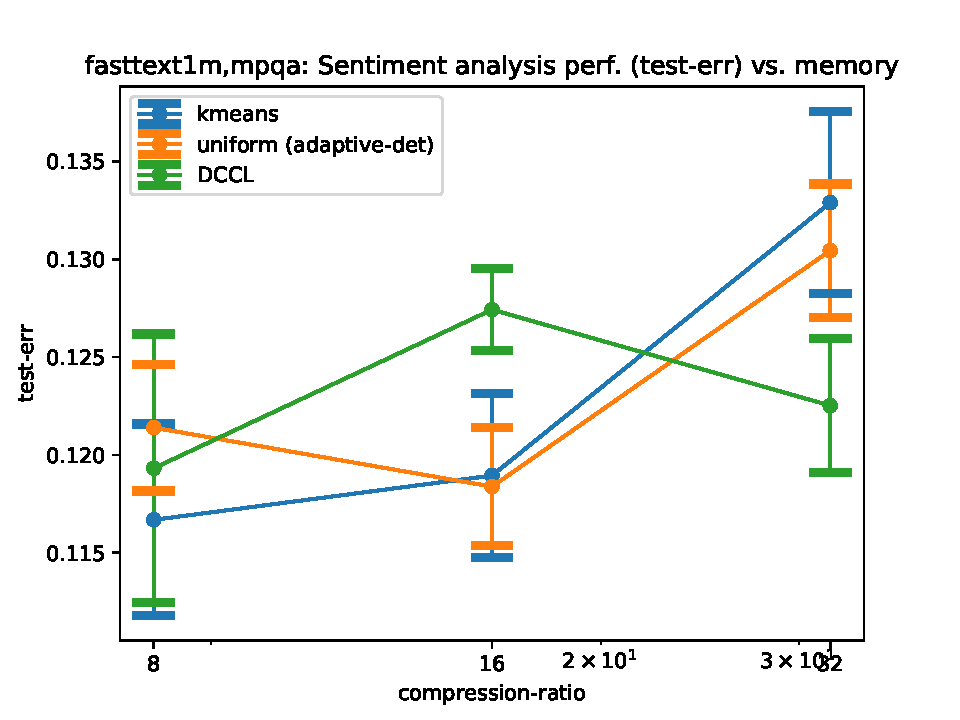
\includegraphics[width=0.28\linewidth]{figures/fasttext1m_mpqa_test-err_vs_compression.pdf} &
%	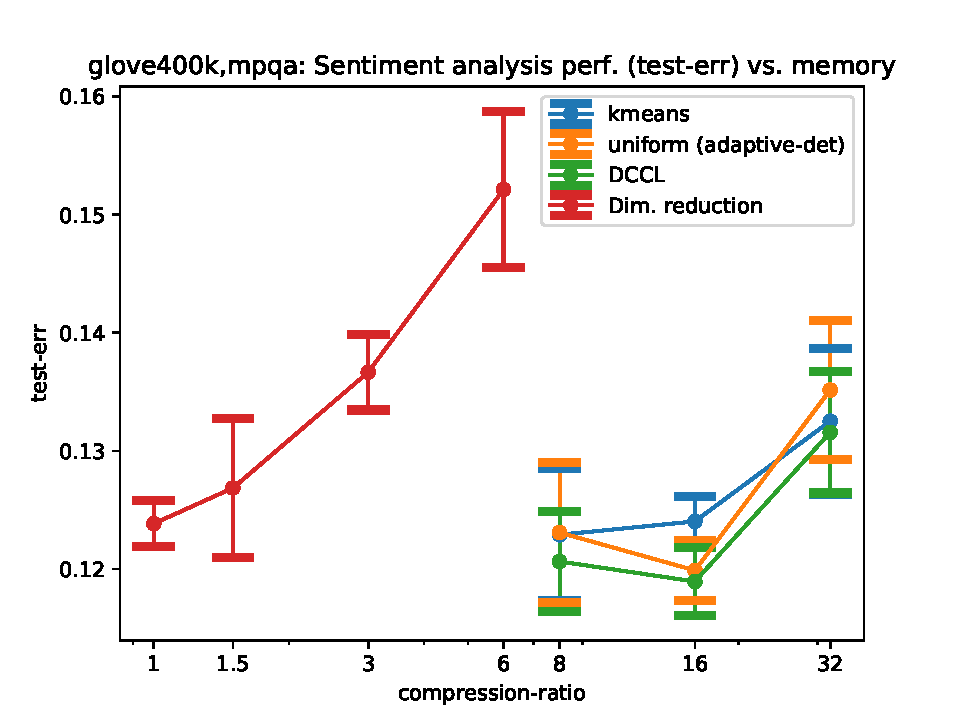
\includegraphics[width=0.28\linewidth]{figures/glove400k_mpqa_test-err_vs_compression.pdf} &
%	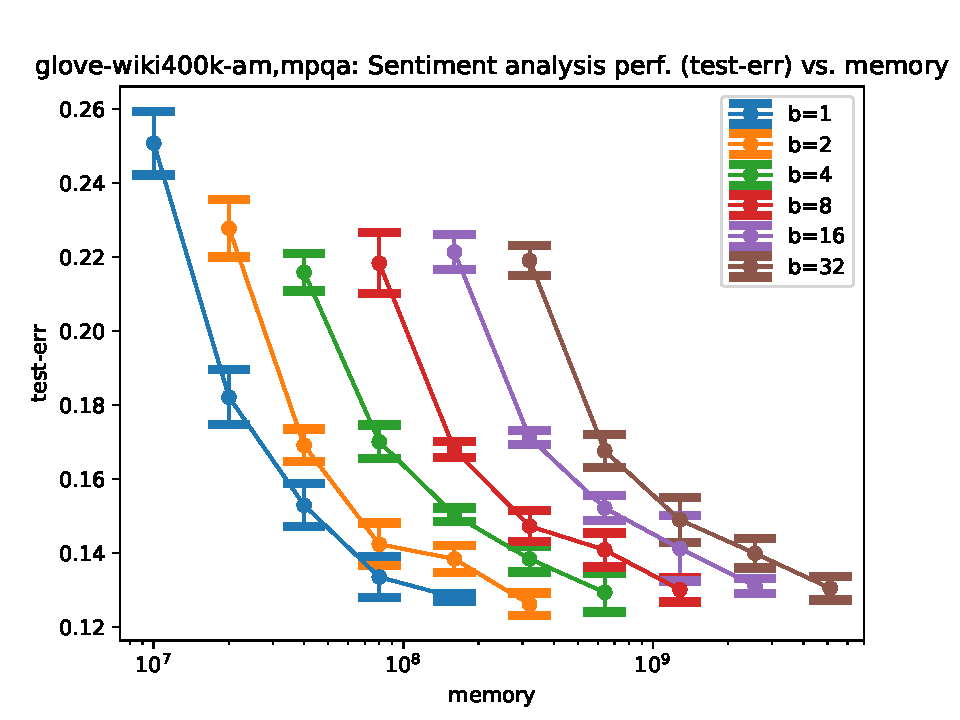
\includegraphics[width=0.28\linewidth]{figures/glove-wiki400k-am_mpqa_test-err_vs_compression.pdf} \\[-0.5em]
%	% TREC
%	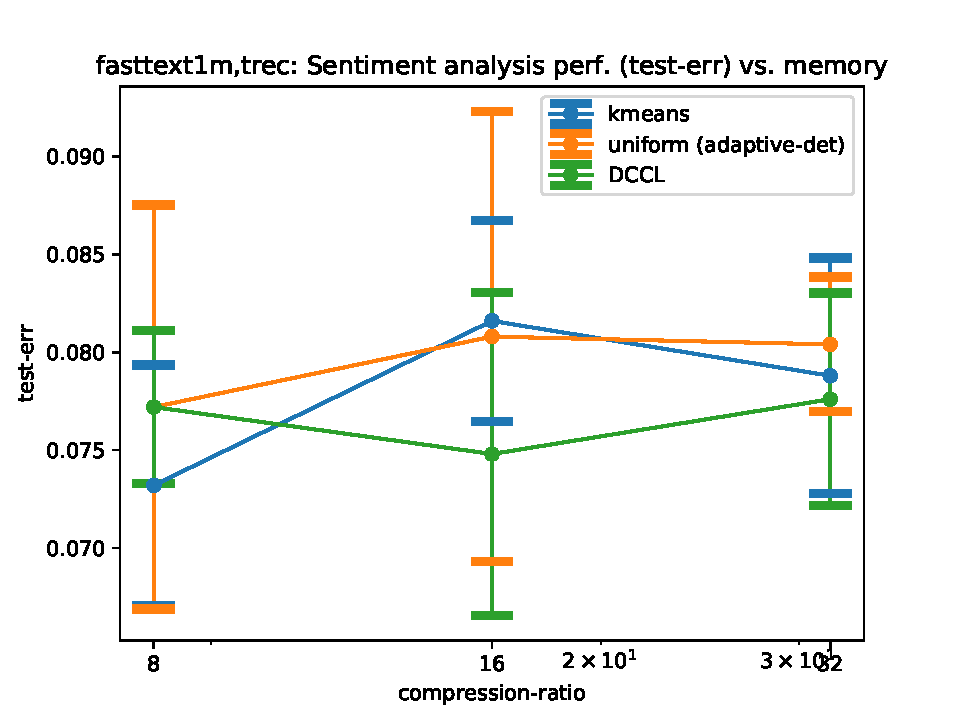
\includegraphics[width=0.28\linewidth]{figures/fasttext1m_trec_test-err_vs_compression.pdf} &
%	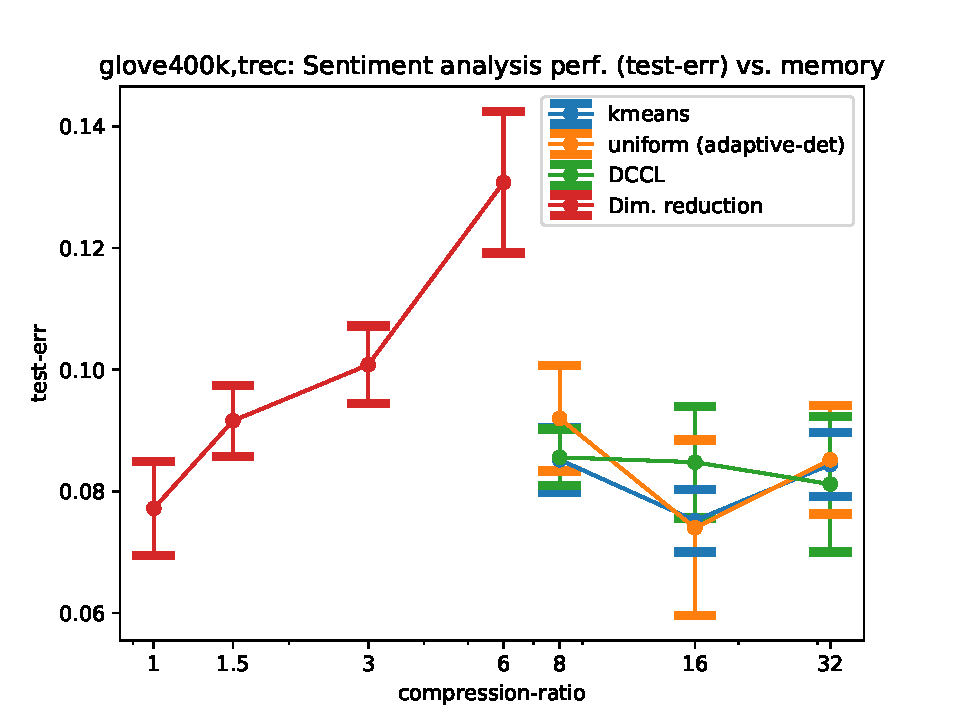
\includegraphics[width=0.28\linewidth]{figures/glove400k_trec_test-err_vs_compression.pdf} &
%	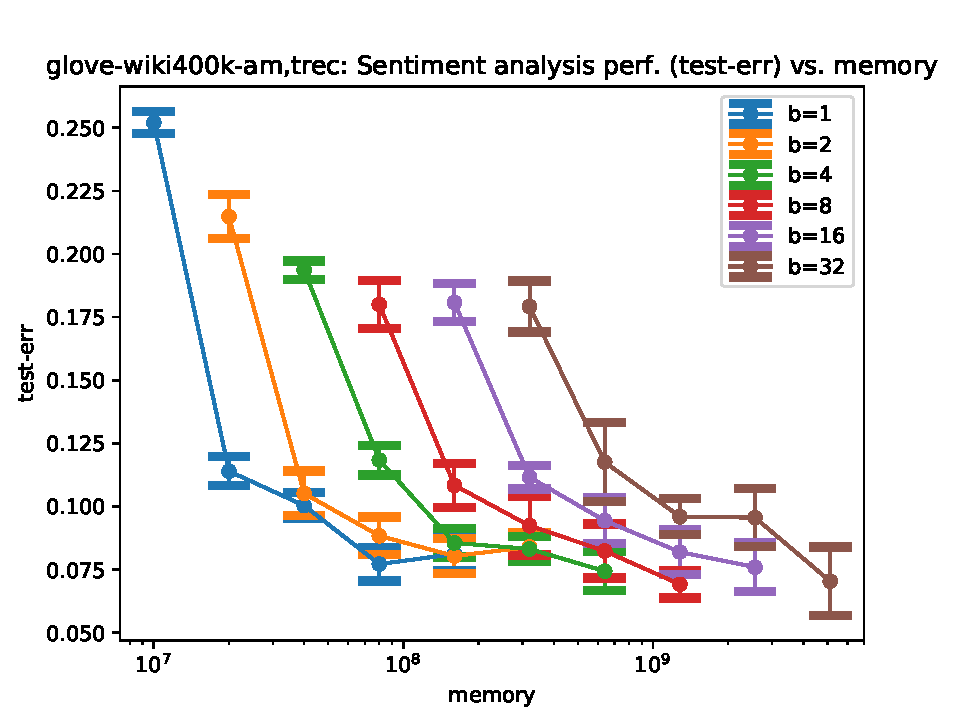
\includegraphics[width=0.28\linewidth]{figures/glove-wiki400k-am_trec_test-err_vs_compression.pdf} \\[-0.5em]
%	% SST
%	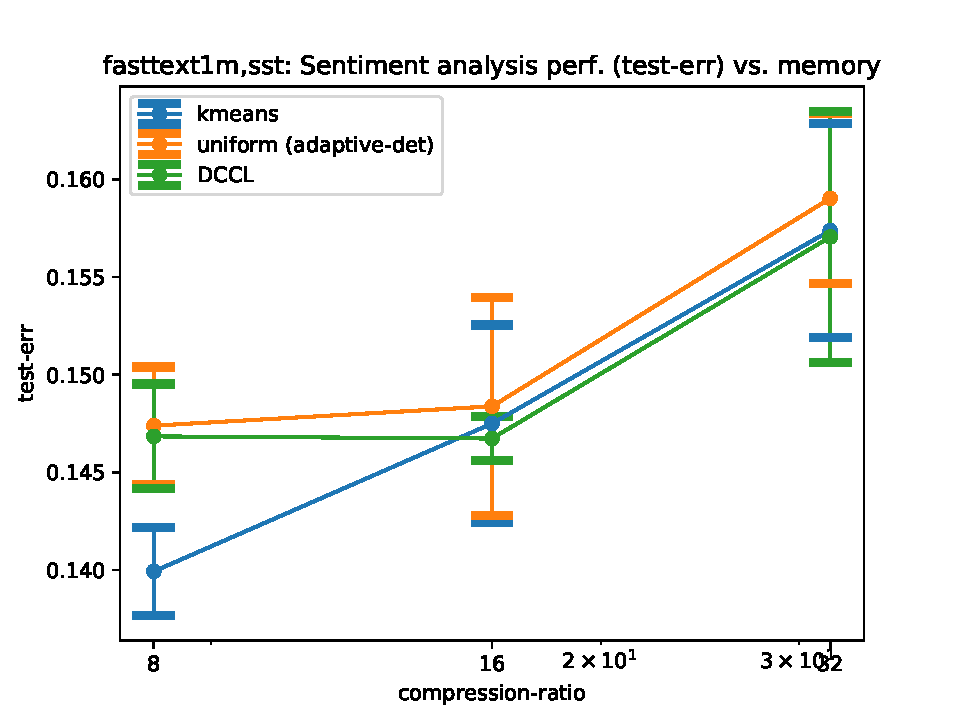
\includegraphics[width=0.28\linewidth]{figures/fasttext1m_sst_test-err_vs_compression.pdf} &
%	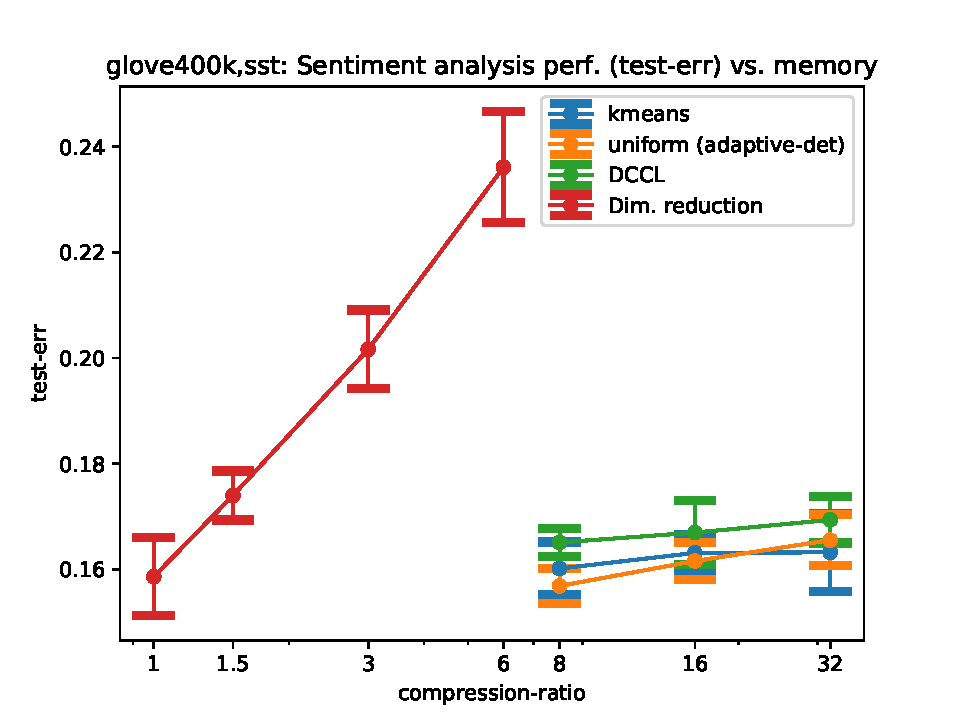
\includegraphics[width=0.28\linewidth]{figures/glove400k_sst_test-err_vs_compression.pdf} &
%	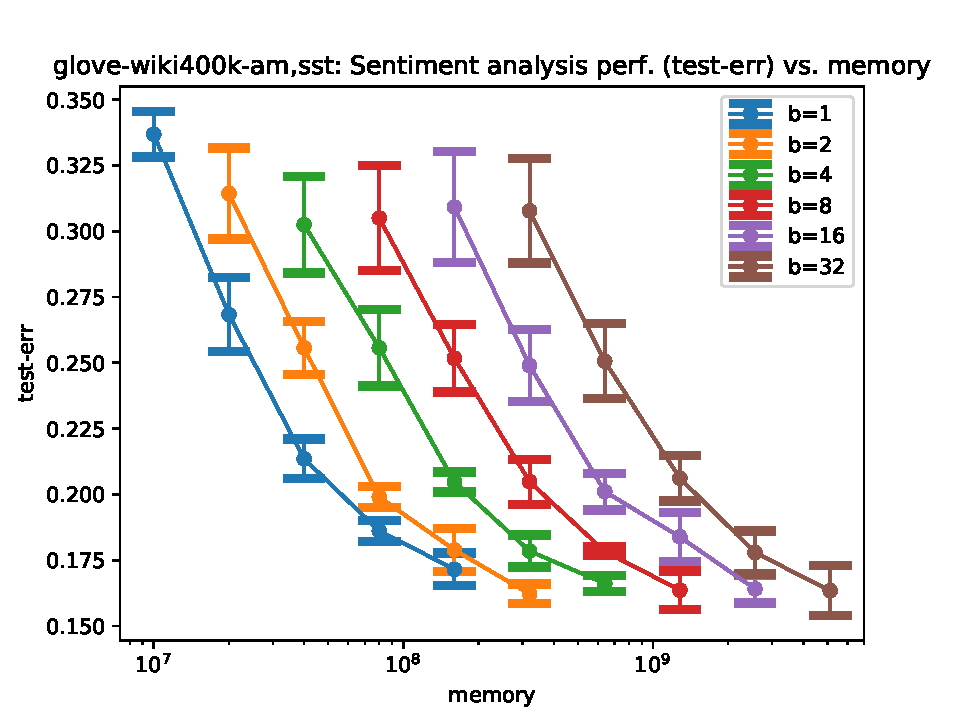
\includegraphics[width=0.28\linewidth]{figures/glove-wiki400k-am_sst_test-err_vs_compression.pdf} \\[-0.5em]
%	% CR
%	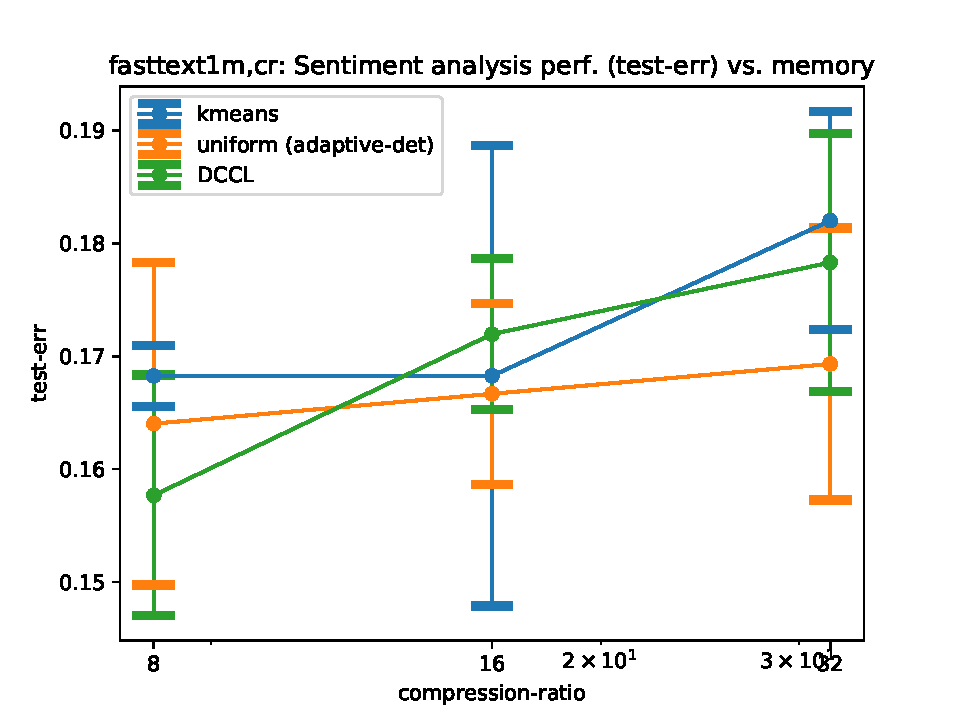
\includegraphics[width=0.28\linewidth]{figures/fasttext1m_cr_test-err_vs_compression.pdf} &
%	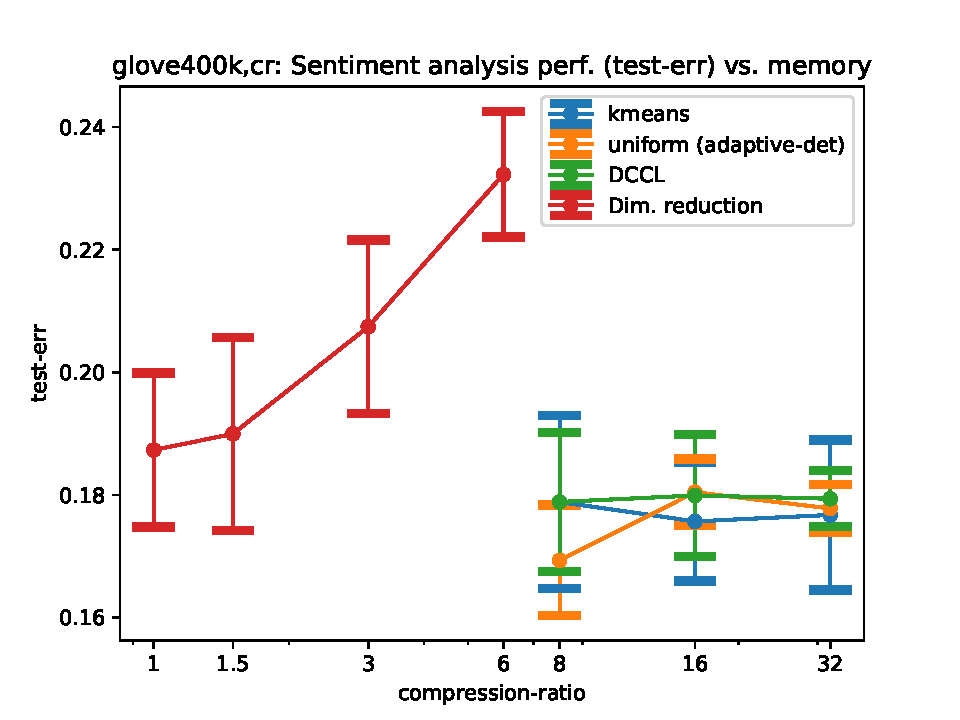
\includegraphics[width=0.28\linewidth]{figures/glove400k_cr_test-err_vs_compression.pdf} &
%	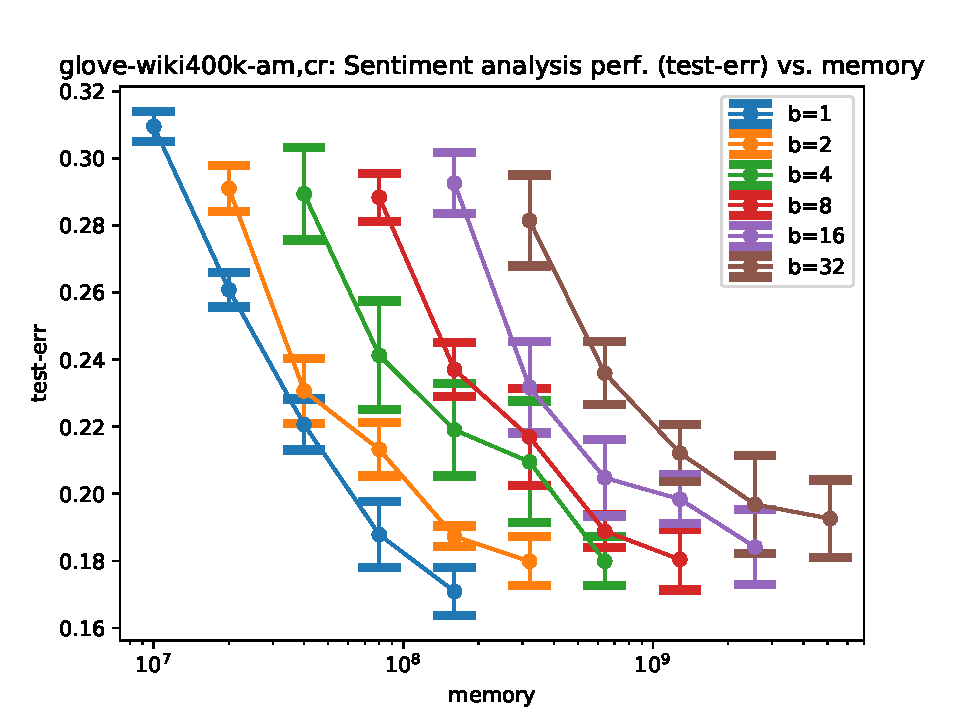
\includegraphics[width=0.28\linewidth]{figures/glove-wiki400k-am_cr_test-err_vs_compression.pdf} \\[-0.5em]
%	% SUBJ
%	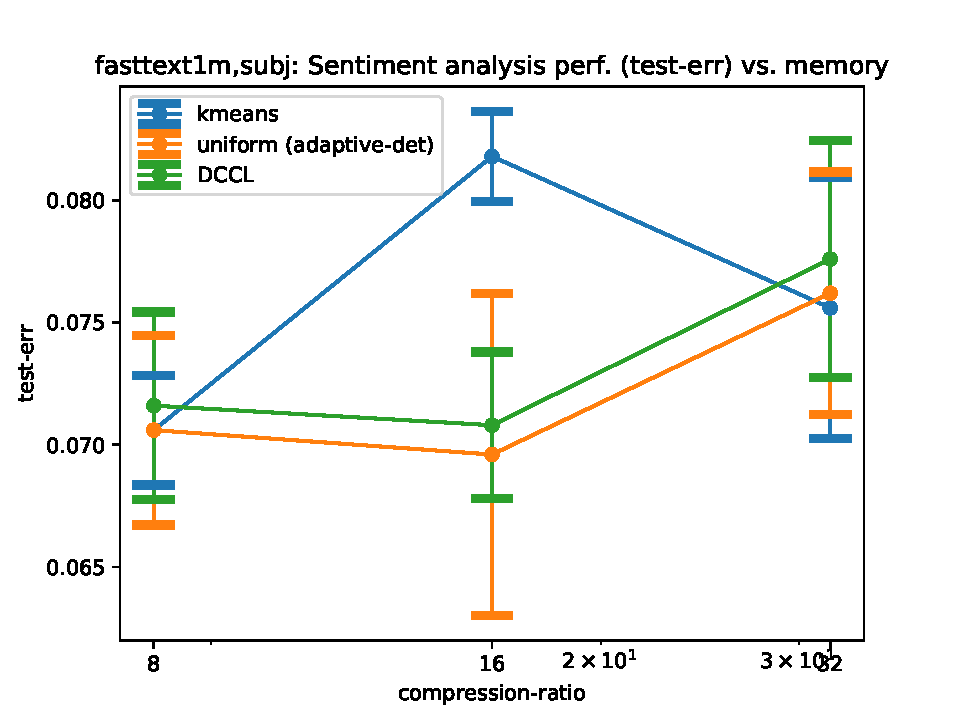
\includegraphics[width=0.28\linewidth]{figures/fasttext1m_subj_test-err_vs_compression.pdf} &
%	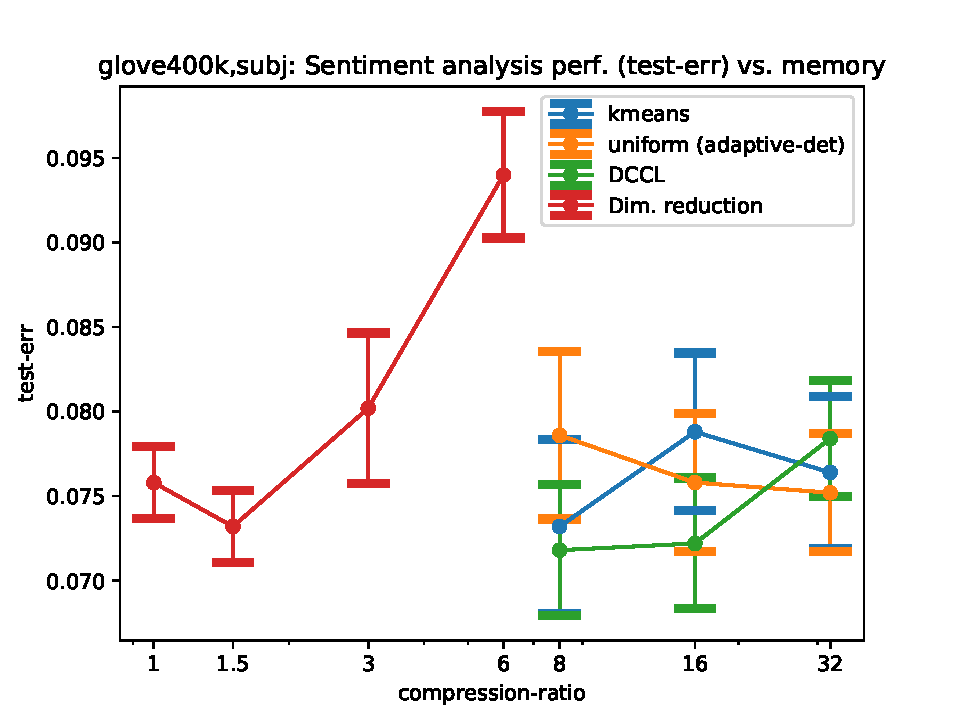
\includegraphics[width=0.28\linewidth]{figures/glove400k_subj_test-err_vs_compression.pdf} &
%	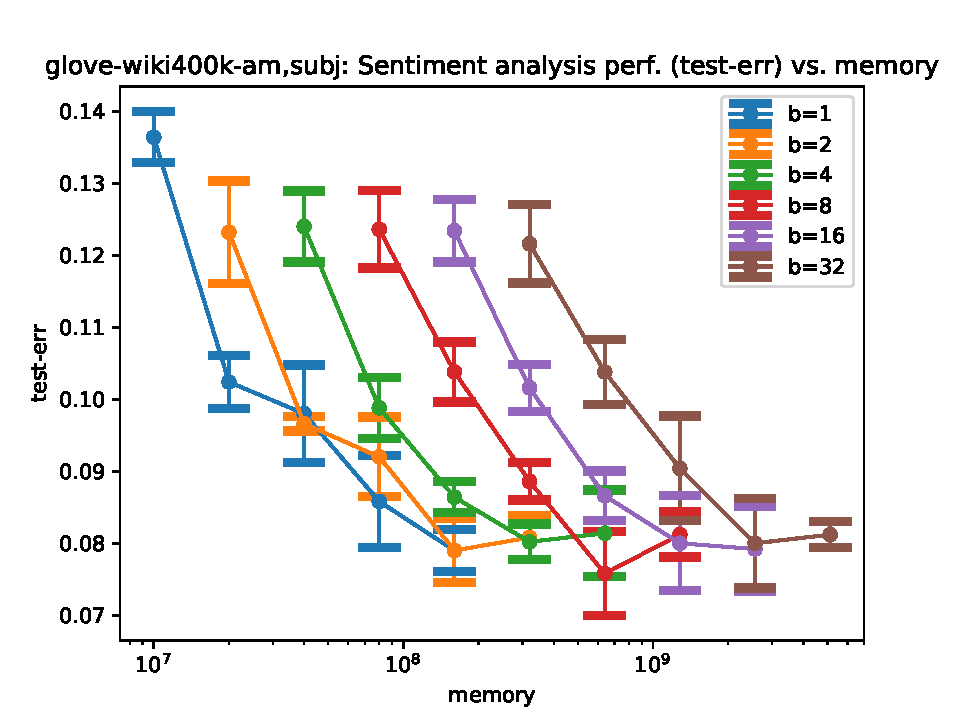
\includegraphics[width=0.28\linewidth]{figures/glove-wiki400k-am_subj_test-err_vs_compression.pdf} \\[-0.5em]
%	% MR
%	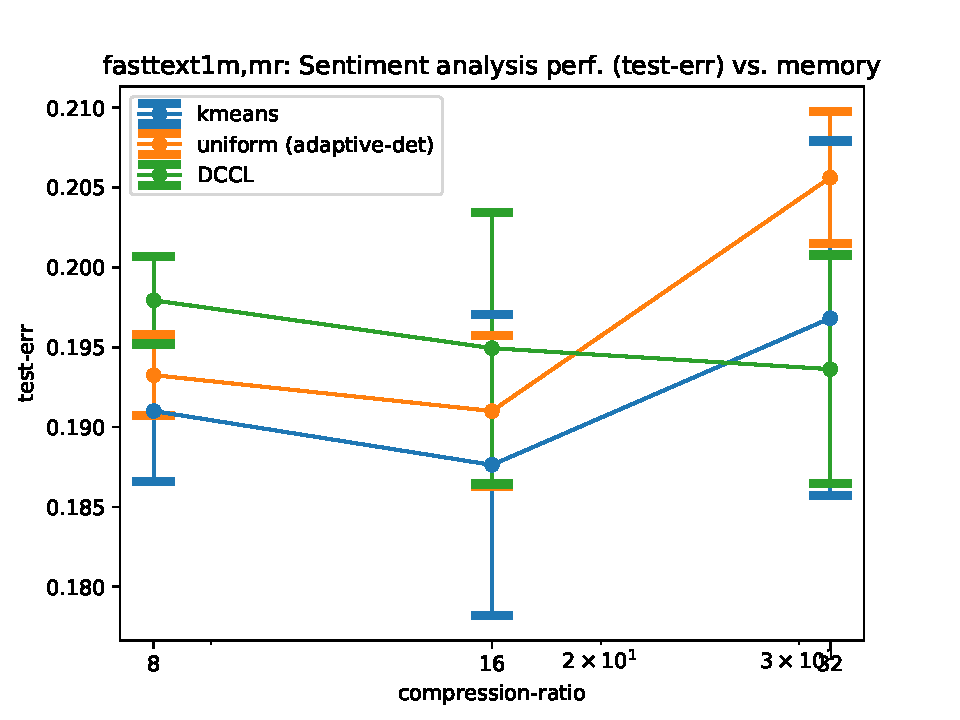
\includegraphics[width=0.28\linewidth]{figures/fasttext1m_mr_test-err_vs_compression.pdf} &
%	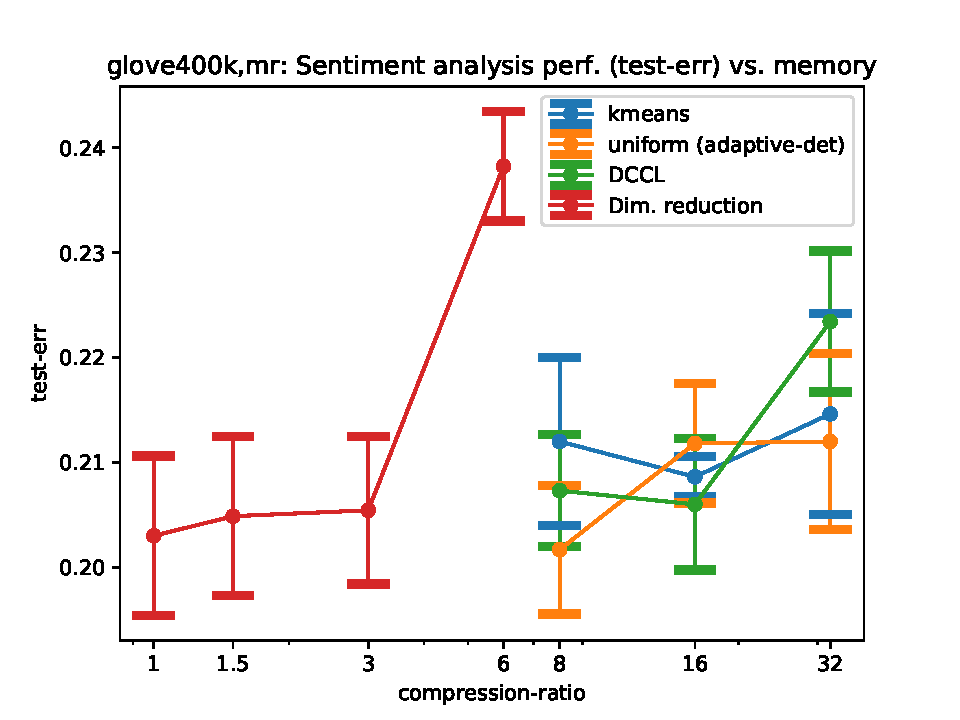
\includegraphics[width=0.28\linewidth]{figures/glove400k_mr_test-err_vs_compression.pdf} &
%	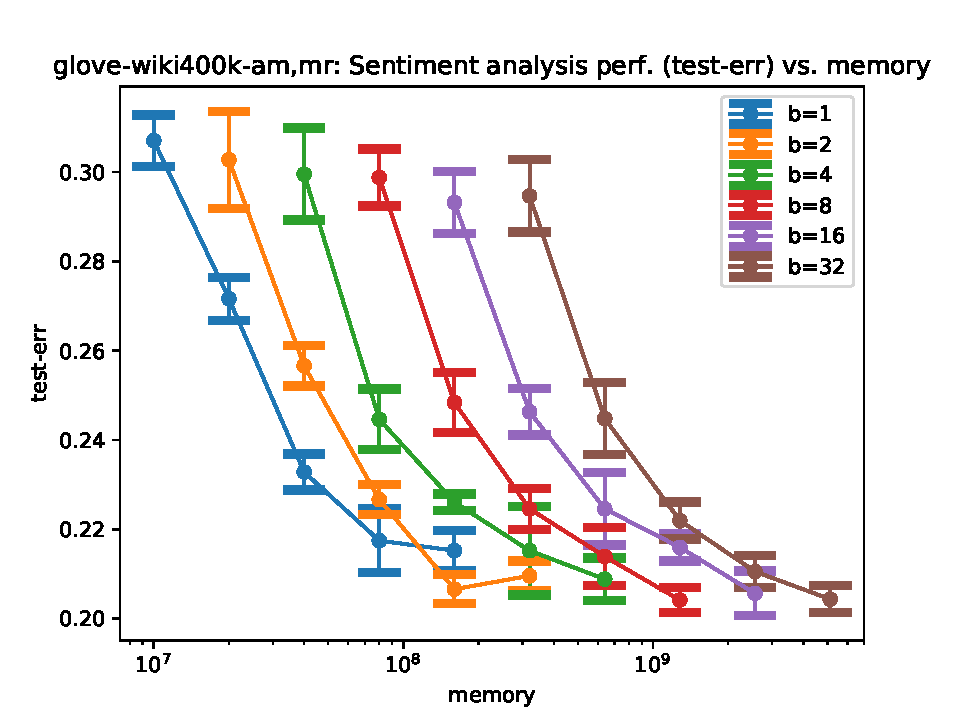
\includegraphics[width=0.28\linewidth]{figures/glove-wiki400k-am_mr_test-err_vs_compression.pdf} \\[-0.5em]
%	\end{tabular}
%	\caption{
%		Sentiment analysis results for different embeddings methods (pre-trained fastText and GloVe embeddings, and GloVe embeddings trained from scratch), on different sentiment analysis datasets (MPQA, TREC, SST, CR, SUBJ, MR).
%	}
%	\label{fig:all_sentiment}
%\end{figure}
%
%\begin{figure*}
%	\centering
%	%	\begin{tabular}{c c c c}
%	\begin{tabular}{@{\hskip -0.0in}c@{\hskip -0.0in}c@{\hskip -0.0in}c@{\hskip -0.0in}c@{\hskip -0.0in}}
%		EIG-OVERLAP & . & . & . \\
%		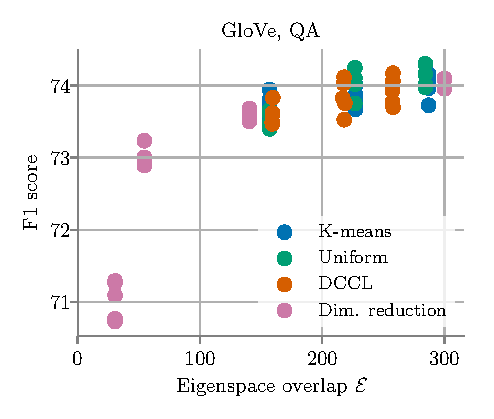
\includegraphics[width=.245\linewidth]{figures/glove400k_qa_best-f1_vs_subspace-eig-overlap_linx.pdf} &
%		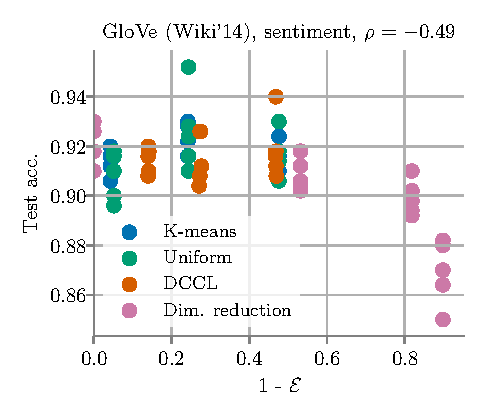
\includegraphics[width=.245\linewidth]{figures/glove400k_sentiment_trec_test-acc_vs_subspace-eig-overlap_linx.pdf} &
%		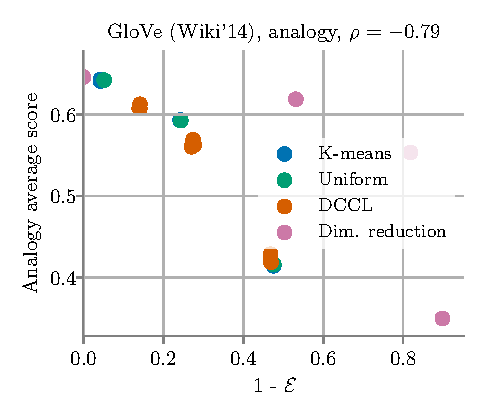
\includegraphics[width=.245\linewidth]{figures/glove400k_intrinsics_analogy-avg-score_vs_subspace-eig-overlap_linx.pdf} &
%		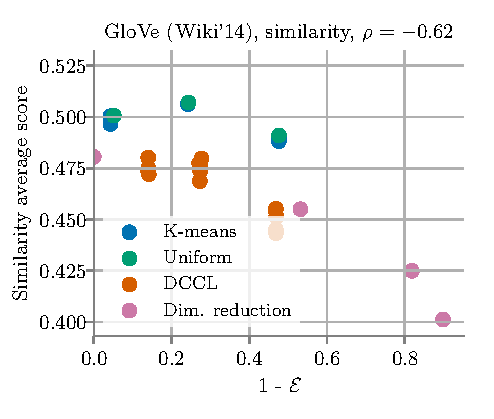
\includegraphics[width=.245\linewidth]{figures/glove400k_intrinsics_similarity-avg-score_vs_subspace-eig-overlap_linx.pdf} \\
%		
%		EIG-DISTANCE & . & . & . \\
%		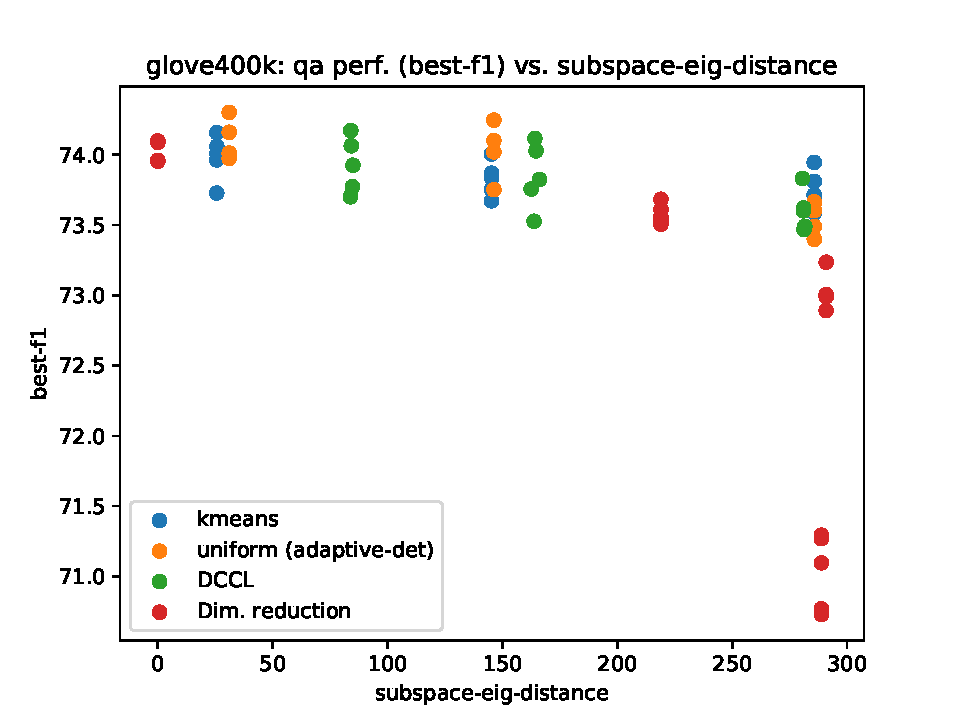
\includegraphics[width=.245\linewidth]{figures/glove400k_qa_best-f1_vs_subspace-eig-distance_linx.pdf} &
%		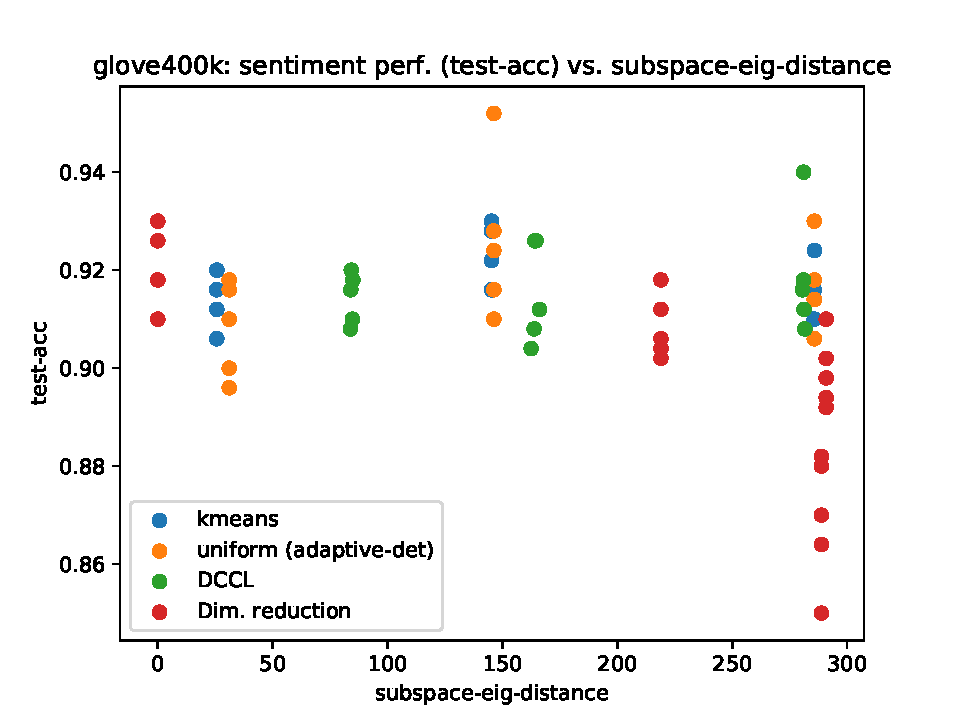
\includegraphics[width=.245\linewidth]{figures/glove400k_sentiment_trec_test-acc_vs_subspace-eig-distance_linx.pdf} &
%		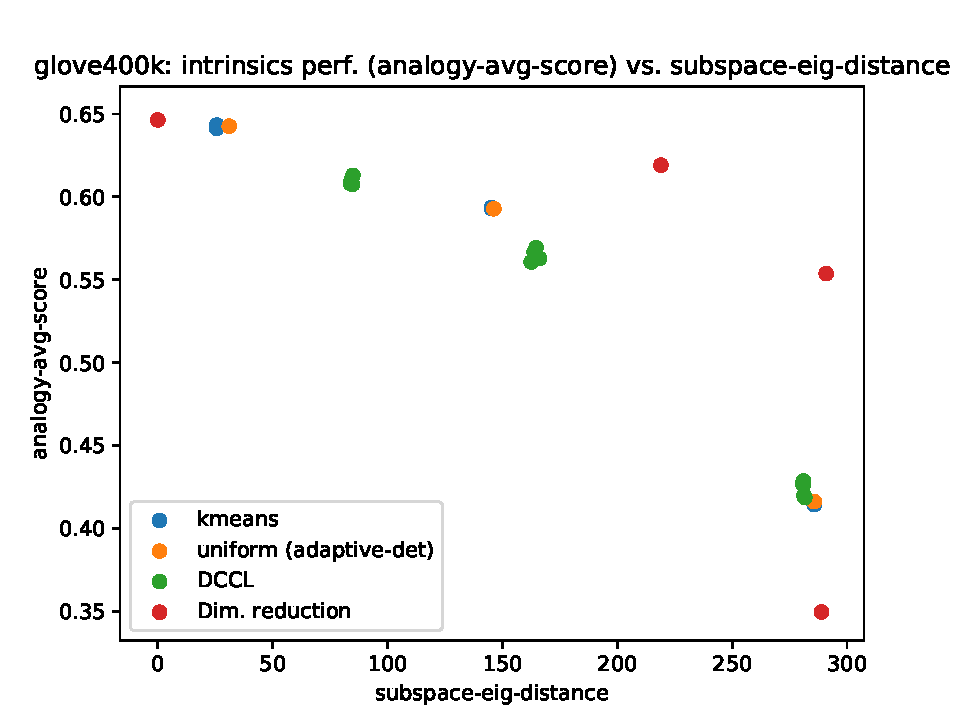
\includegraphics[width=.245\linewidth]{figures/glove400k_intrinsics_analogy-avg-score_vs_subspace-eig-distance_linx.pdf} &
%		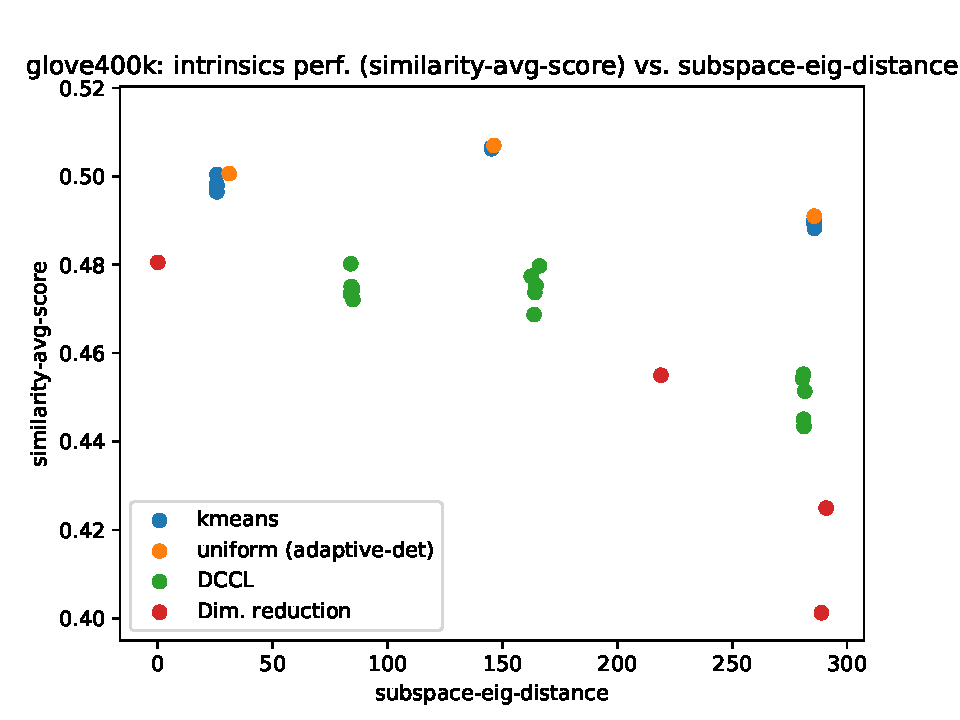
\includegraphics[width=.245\linewidth]{figures/glove400k_intrinsics_similarity-avg-score_vs_subspace-eig-distance_linx.pdf} \\
%		
%		FROBENIUS ERROR & . & . & . \\		
%		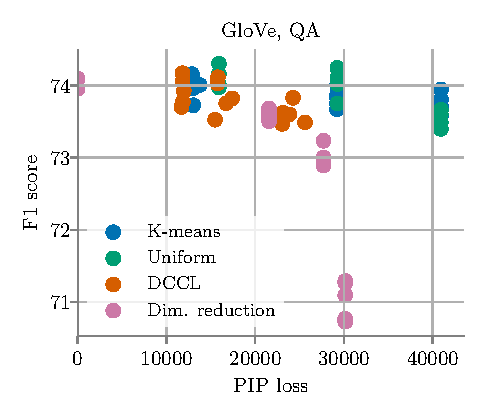
\includegraphics[width=.245\linewidth]{figures/glove400k_qa_best-f1_vs_gram-large-dim-frob-error_linx.pdf} &
%		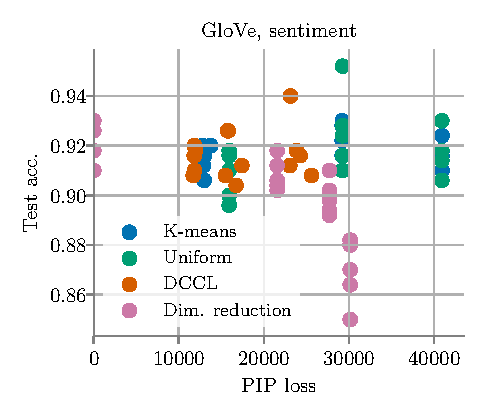
\includegraphics[width=.245\linewidth]{figures/glove400k_sentiment_trec_test-acc_vs_gram-large-dim-frob-error_linx.pdf} &
%		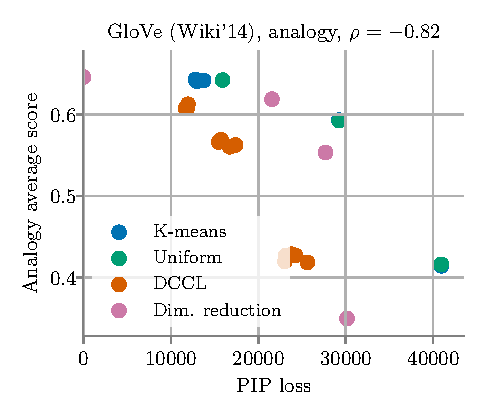
\includegraphics[width=.245\linewidth]{figures/glove400k_intrinsics_analogy-avg-score_vs_gram-large-dim-frob-error_linx.pdf} &
%		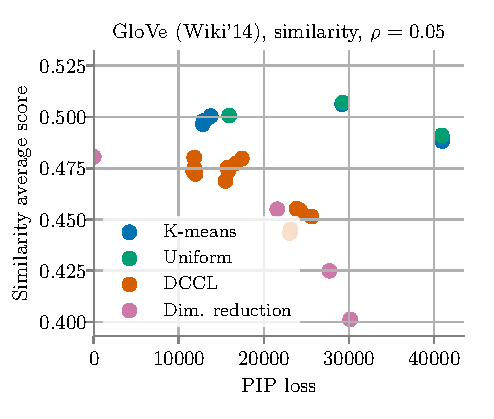
\includegraphics[width=.245\linewidth]{figures/glove400k_intrinsics_similarity-avg-score_vs_gram-large-dim-frob-error_linx.pdf} \\
%		
%		RECONSTRUCTION ERROR (FROB) & . & . & . \\		
%		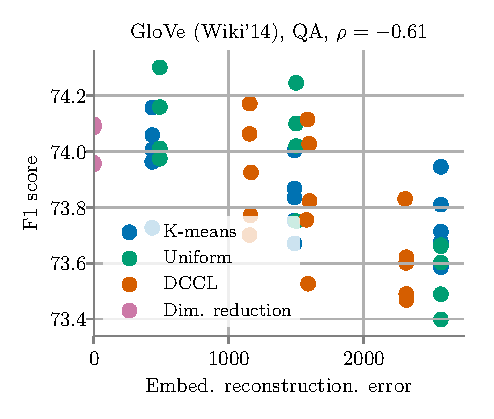
\includegraphics[width=.245\linewidth]{figures/glove400k_qa_best-f1_vs_embed-frob-error_linx.pdf} &
%		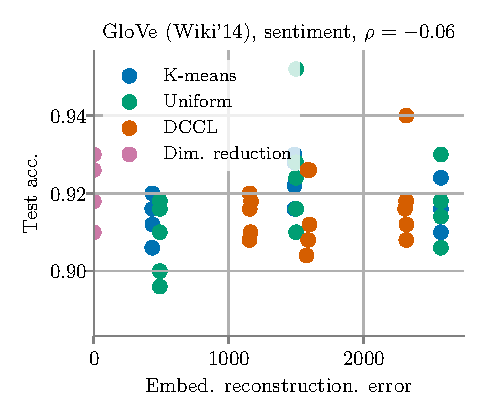
\includegraphics[width=.245\linewidth]{figures/glove400k_sentiment_trec_test-acc_vs_embed-frob-error_linx.pdf} &
%		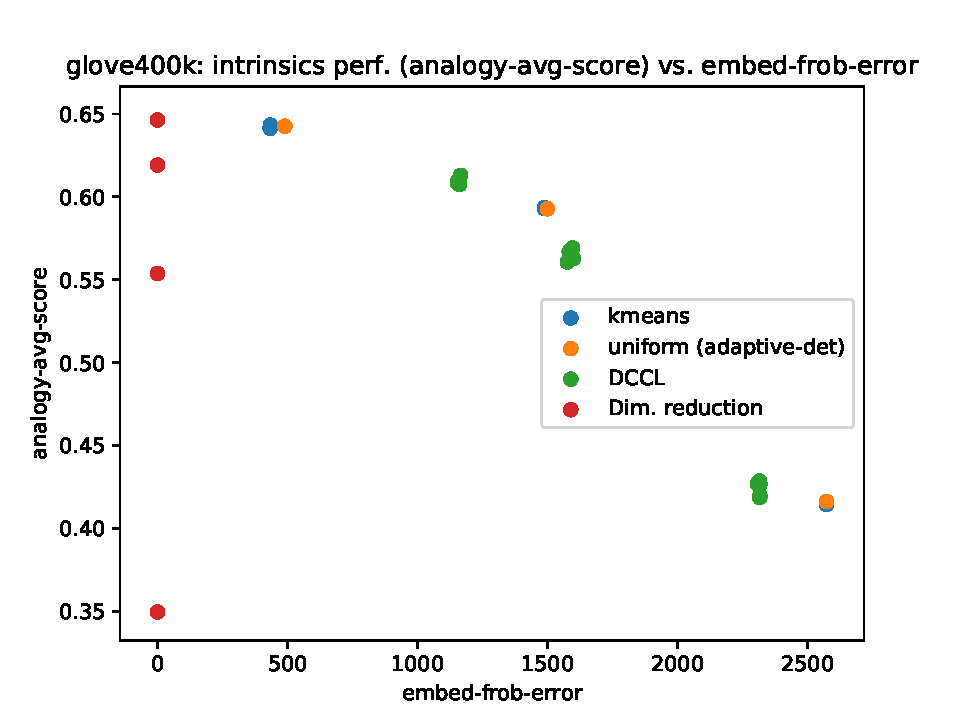
\includegraphics[width=.245\linewidth]{figures/glove400k_intrinsics_analogy-avg-score_vs_embed-frob-error_linx.pdf} &
%		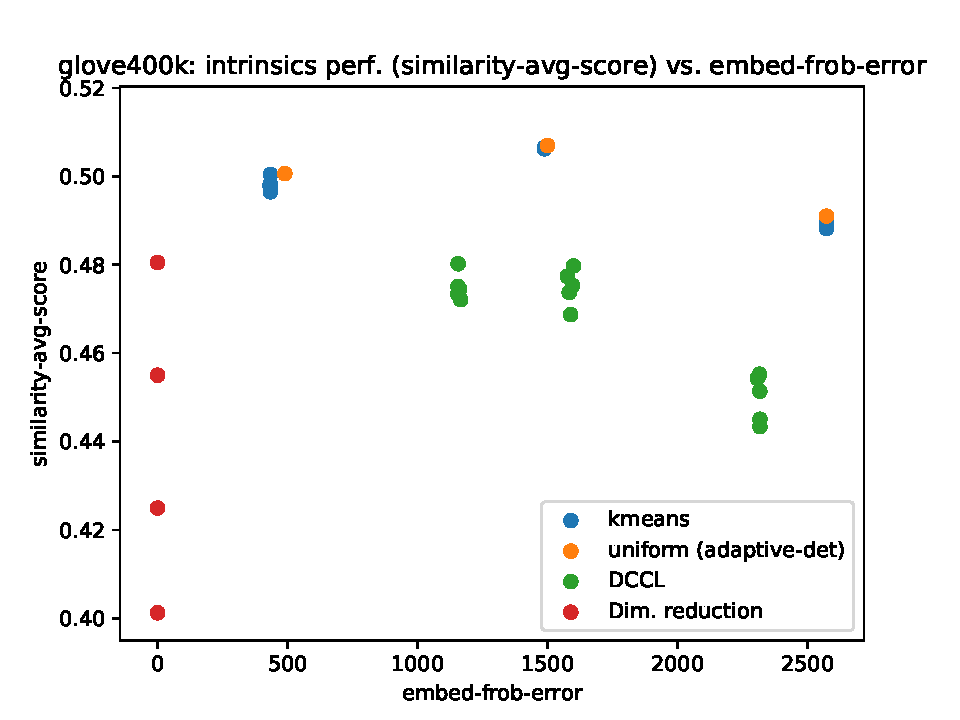
\includegraphics[width=.245\linewidth]{figures/glove400k_intrinsics_similarity-avg-score_vs_embed-frob-error_linx.pdf} \\
%		
%		
%		%DELTA1 (Lambda = sigma min/100) & . & . & . \\
%		%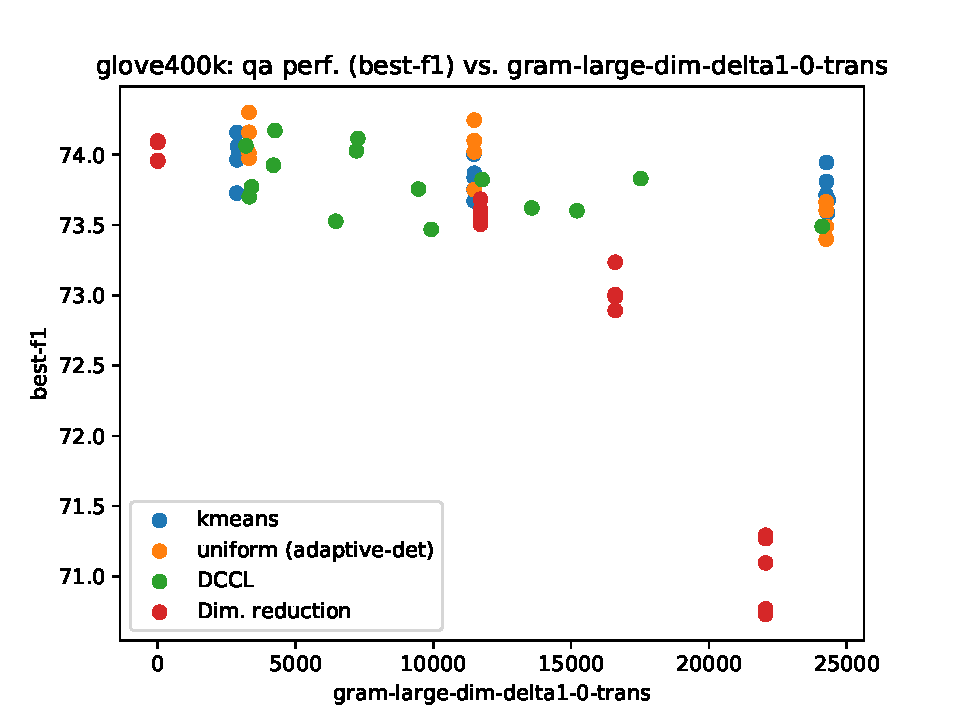
\includegraphics[width=.245\linewidth]{figures/glove400k_qa_best-f1_vs_gram-large-dim-delta1-0-trans_linx.pdf} &
%		%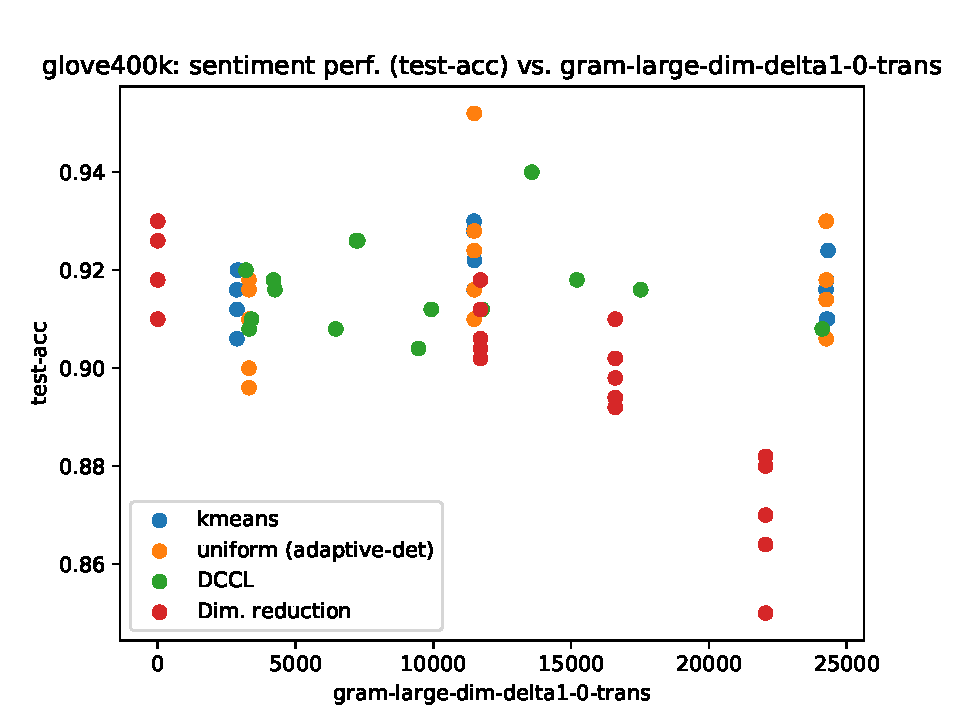
\includegraphics[width=.245\linewidth]{figures/glove400k_sentiment_trec_test-acc_vs_gram-large-dim-delta1-0-trans_linx.pdf} &
%		%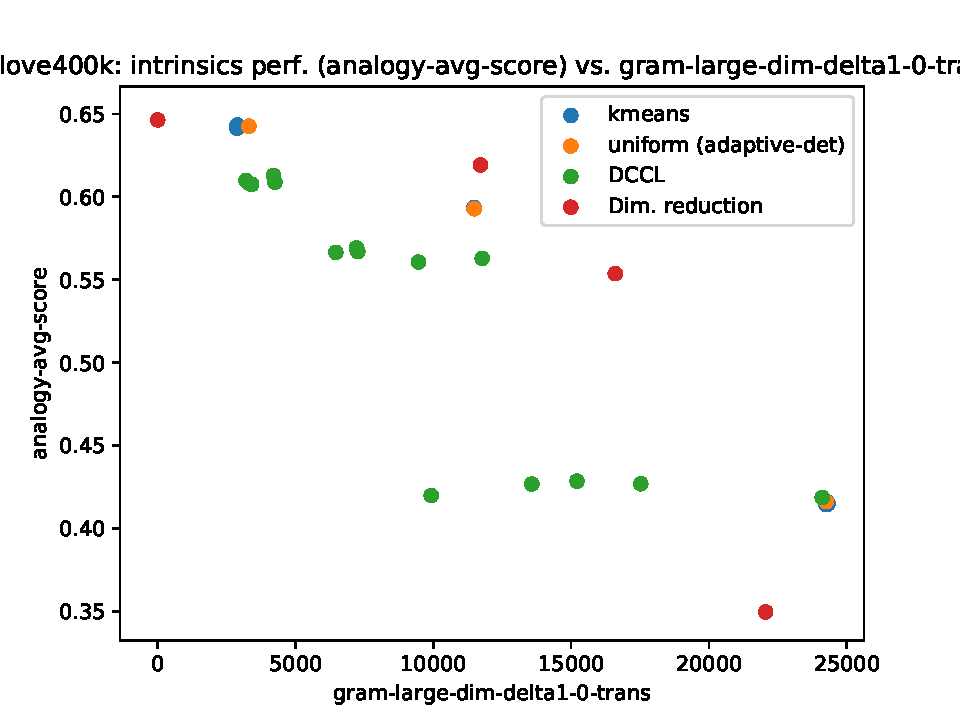
\includegraphics[width=.245\linewidth]{figures/glove400k_intrinsics_analogy-avg-score_vs_gram-large-dim-delta1-0-trans_linx.pdf} &
%		%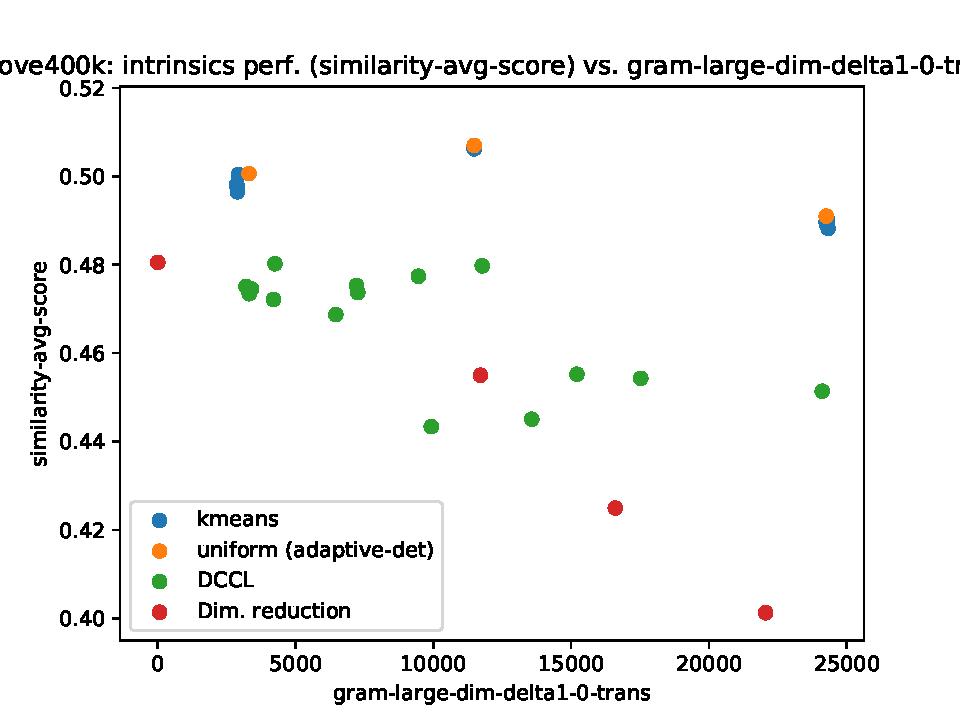
\includegraphics[width=.245\linewidth]{figures/glove400k_intrinsics_similarity-avg-score_vs_gram-large-dim-delta1-0-trans_linx.pdf} \\
%		
%		DELTA1 (Lambda = sigma min) & . & . & . \\
%		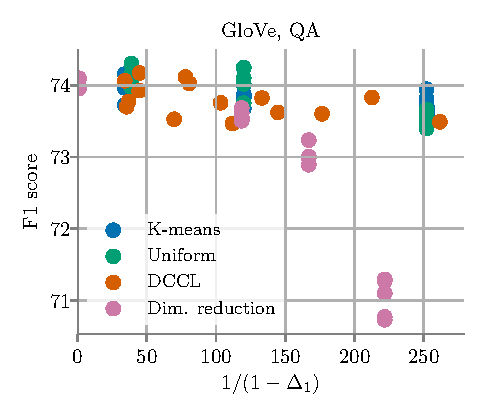
\includegraphics[width=.245\linewidth]{figures/glove400k_qa_best-f1_vs_gram-large-dim-delta1-2-trans_linx.pdf} &
%		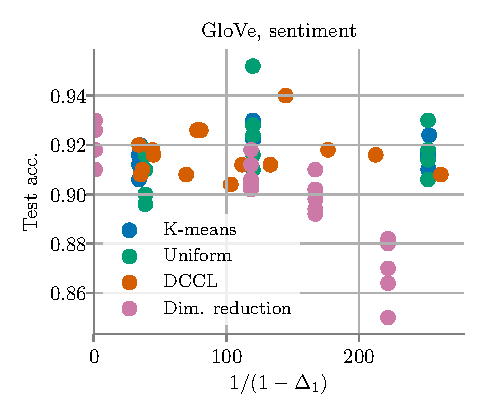
\includegraphics[width=.245\linewidth]{figures/glove400k_sentiment_trec_test-acc_vs_gram-large-dim-delta1-2-trans_linx.pdf} &
%		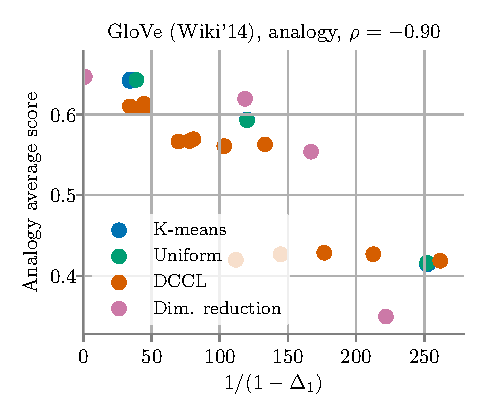
\includegraphics[width=.245\linewidth]{figures/glove400k_intrinsics_analogy-avg-score_vs_gram-large-dim-delta1-2-trans_linx.pdf} &
%		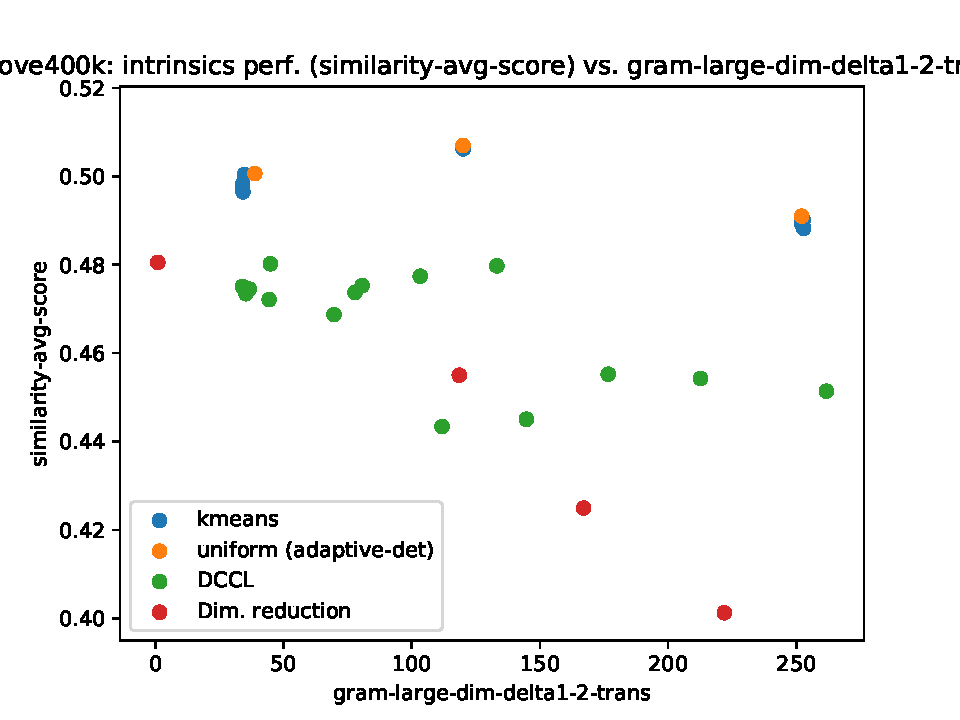
\includegraphics[width=.245\linewidth]{figures/glove400k_intrinsics_similarity-avg-score_vs_gram-large-dim-delta1-2-trans_linx.pdf} \\		
%		
%		DELTA1 (lambda = sigma max) & . & . & . \\
%		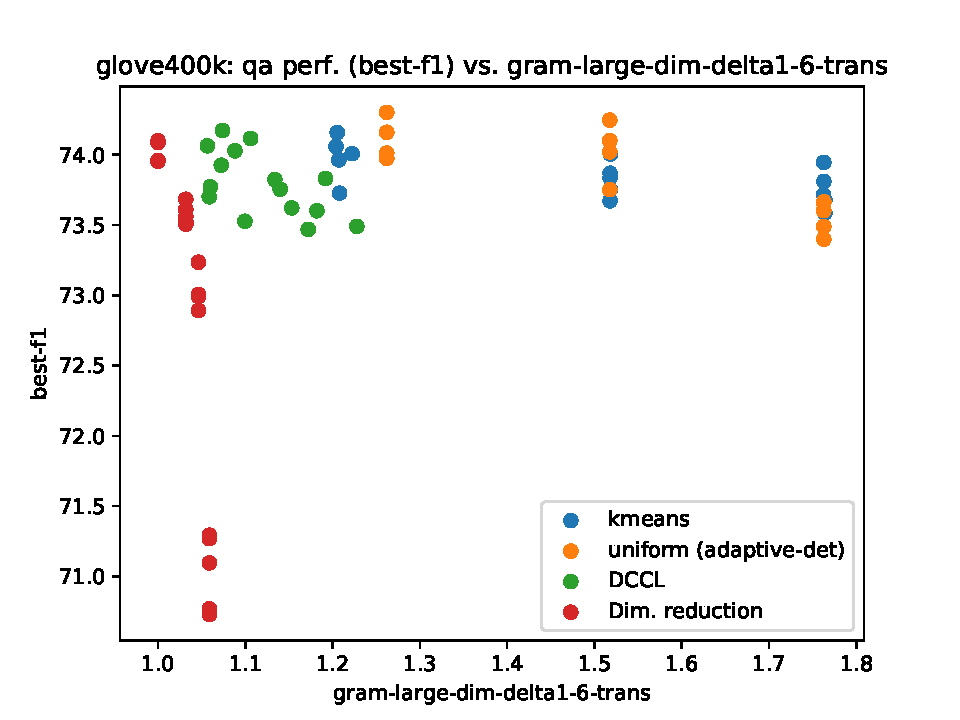
\includegraphics[width=.245\linewidth]{figures/glove400k_qa_best-f1_vs_gram-large-dim-delta1-6-trans_linx.pdf} &
%		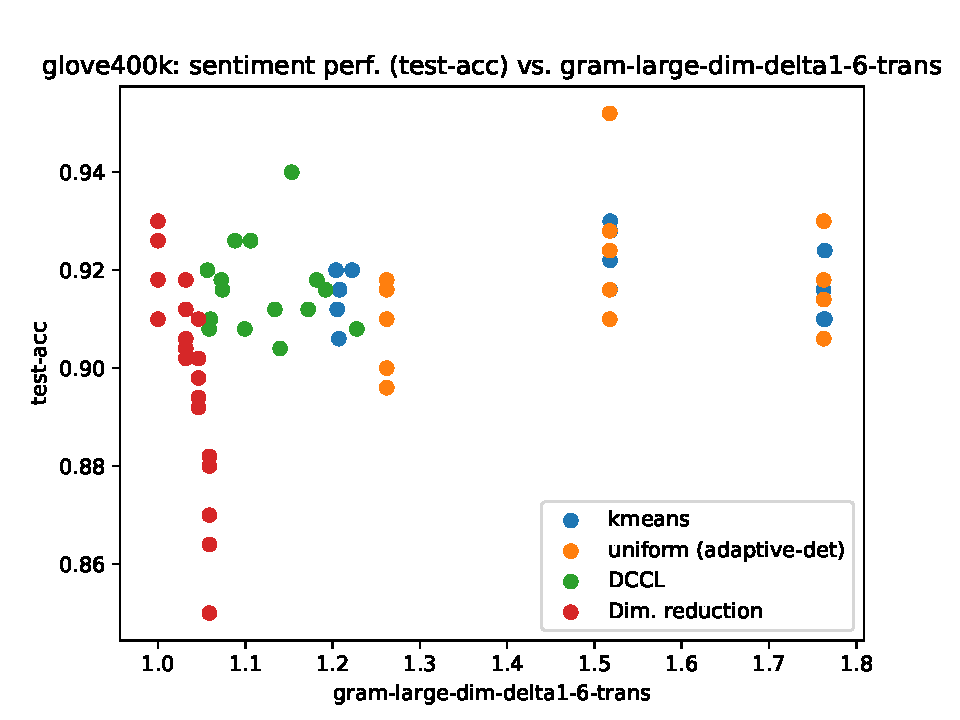
\includegraphics[width=.245\linewidth]{figures/glove400k_sentiment_trec_test-acc_vs_gram-large-dim-delta1-6-trans_linx.pdf} &
%		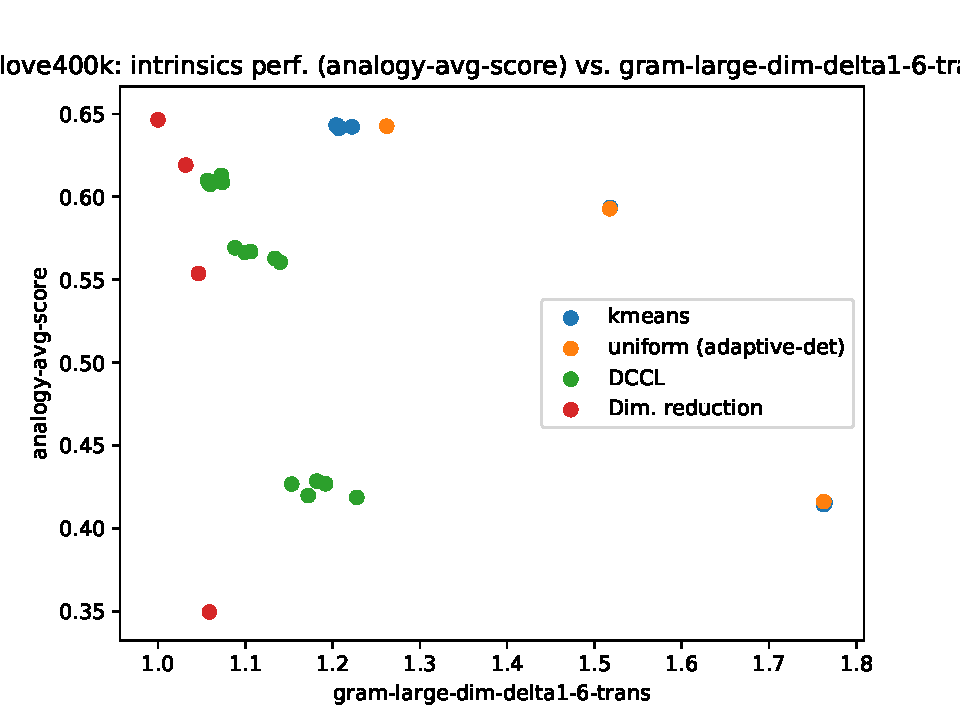
\includegraphics[width=.245\linewidth]{figures/glove400k_intrinsics_analogy-avg-score_vs_gram-large-dim-delta1-6-trans_linx.pdf} &
%		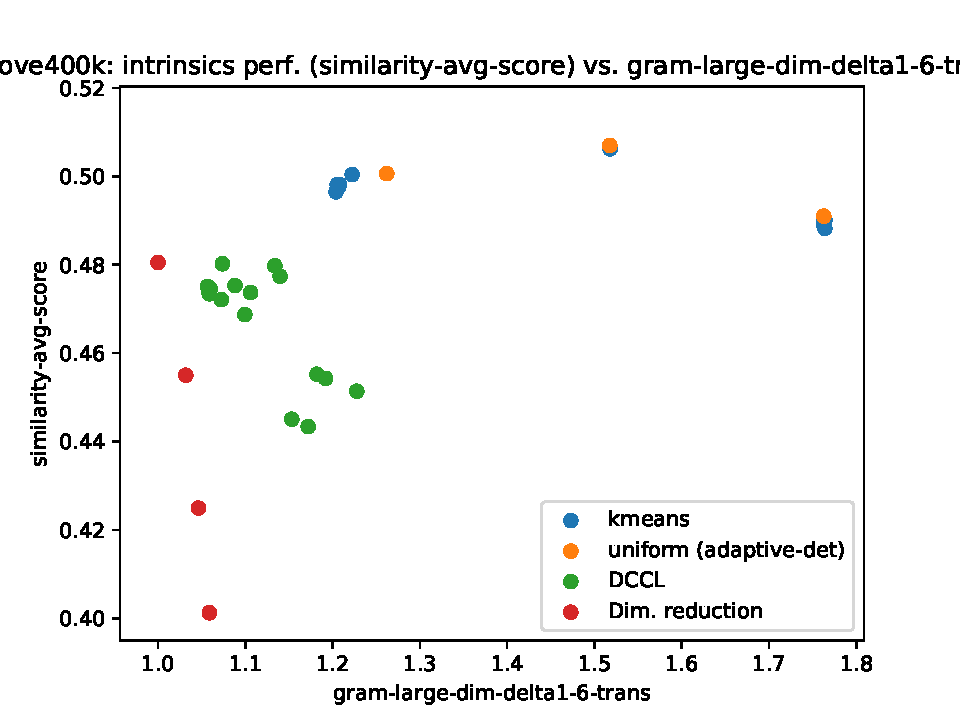
\includegraphics[width=.245\linewidth]{figures/glove400k_intrinsics_similarity-avg-score_vs_gram-large-dim-delta1-6-trans_linx.pdf} \\		
%		
%		\;\;\;\;\;(a) & \;\;\;\;\;\;(b) & \;\;\;\;\;\;(c) & \;\;\;\;\;\;(d)
%	\end{tabular}
%	\caption{GLOVE400k: Performance vs. metrics. (a) QA, (b) Sentiment (TREC), (c) Analogy average, (d) Similarity average.
%	}
%	\label{fig:glove400k_comparison_results}
%\end{figure*}
%
%
%\begin{figure*}
%	\centering
%	%	\begin{tabular}{c c c c}
%	\begin{tabular}{@{\hskip -0.0in}c@{\hskip -0.0in}c@{\hskip -0.0in}c@{\hskip -0.0in}c@{\hskip -0.0in}}
%		EIG-OVERLAP & . & . & . \\
%		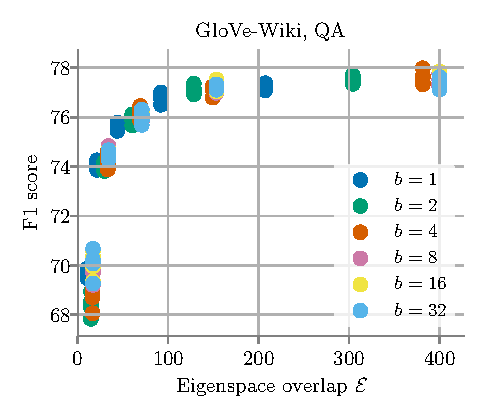
\includegraphics[width=.245\linewidth]{figures/glove-wiki400k-am_qa_best-f1_vs_subspace-eig-overlap_linx.pdf} &
%		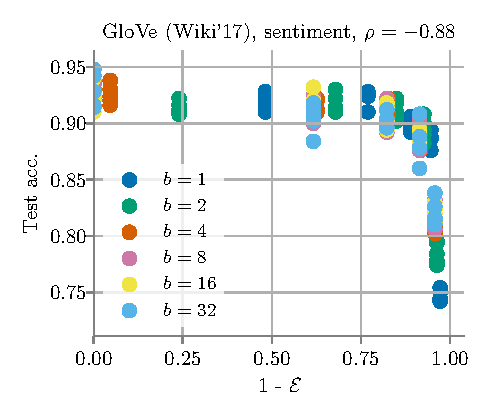
\includegraphics[width=.245\linewidth]{figures/glove-wiki400k-am_sentiment_trec_test-acc_vs_subspace-eig-overlap_linx.pdf} &
%		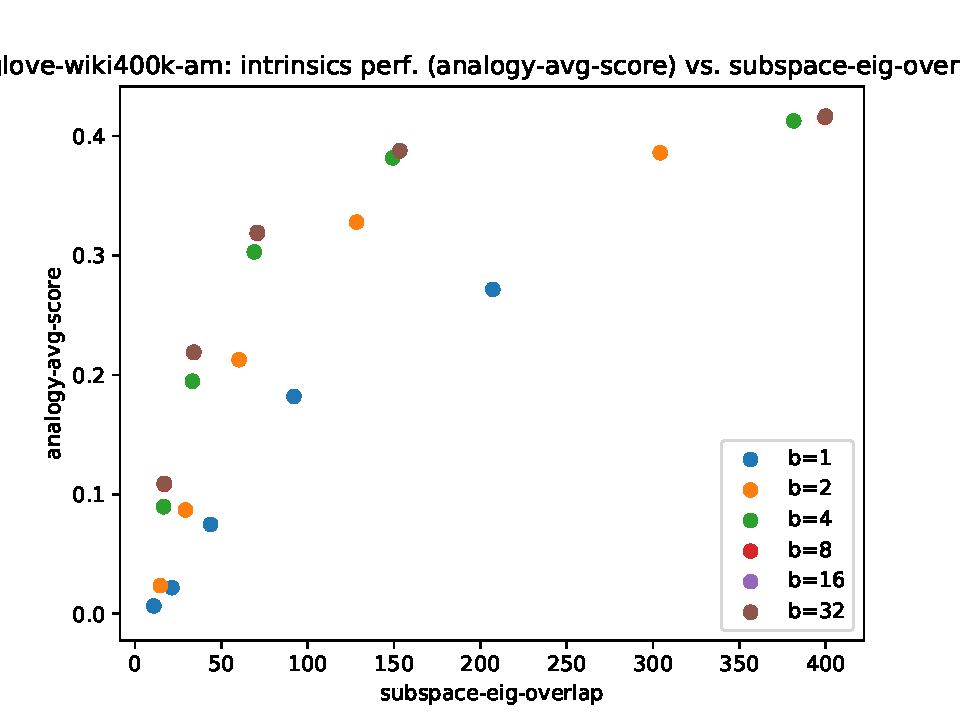
\includegraphics[width=.245\linewidth]{figures/glove-wiki400k-am_intrinsics_analogy-avg-score_vs_subspace-eig-overlap_linx.pdf} &
%		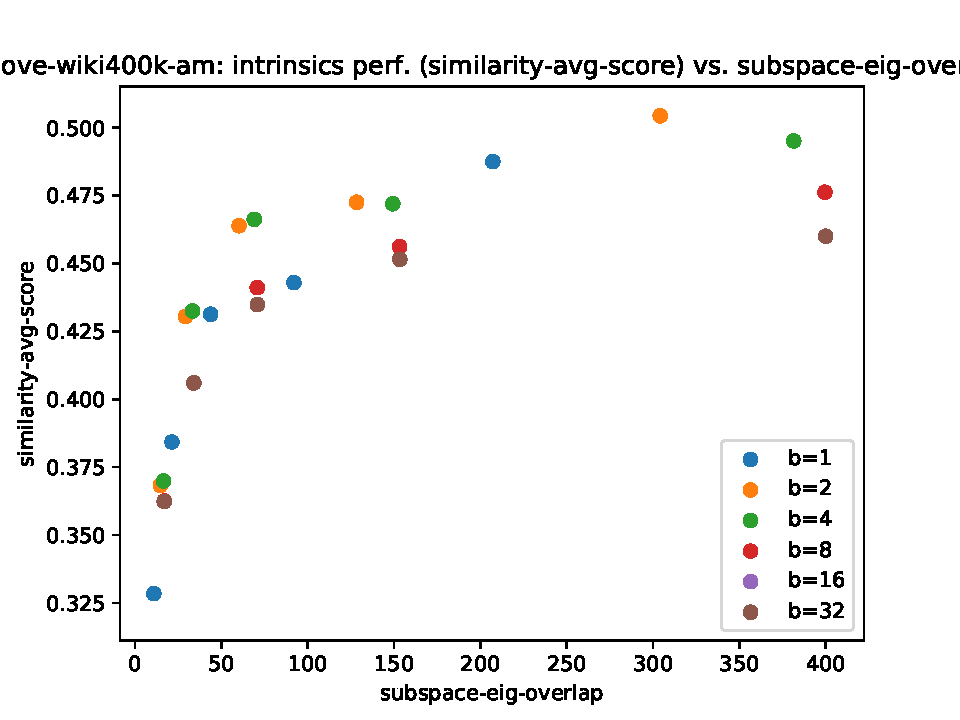
\includegraphics[width=.245\linewidth]{figures/glove-wiki400k-am_intrinsics_similarity-avg-score_vs_subspace-eig-overlap_linx.pdf} \\
%		
%		EIG-DISTANCE & . & . & . \\
%		\includegraphics[width=.245\linewidth]{figures/glove-wiki400k-am_qa_best-f1_vs_subspace-eig-distance_linx.pdf} &
%		\includegraphics[width=.245\linewidth]{figures/glove-wiki400k-am_sentiment_trec_test-acc_vs_subspace-eig-distance_linx.pdf} &
%		\includegraphics[width=.245\linewidth]{figures/glove-wiki400k-am_intrinsics_analogy-avg-score_vs_subspace-eig-distance_linx.pdf} &
%		\includegraphics[width=.245\linewidth]{figures/glove-wiki400k-am_intrinsics_similarity-avg-score_vs_subspace-eig-distance_linx.pdf} \\
%		
%		FROBENIUS ERROR & . & . & . \\		
%		\includegraphics[width=.245\linewidth]{figures/glove-wiki400k-am_qa_best-f1_vs_gram-large-dim-frob-error_linx.pdf} &
%		\includegraphics[width=.245\linewidth]{figures/glove-wiki400k-am_sentiment_trec_test-acc_vs_gram-large-dim-frob-error_linx.pdf} &
%		\includegraphics[width=.245\linewidth]{figures/glove-wiki400k-am_intrinsics_analogy-avg-score_vs_gram-large-dim-frob-error_linx.pdf} &
%		\includegraphics[width=.245\linewidth]{figures/glove-wiki400k-am_intrinsics_similarity-avg-score_vs_gram-large-dim-frob-error_linx.pdf} \\
%		
%		
%		RECONSTRUCTION ERROR (FROB) & . & . & . \\		
%		\includegraphics[width=.245\linewidth]{figures/glove-wiki400k-am_qa_best-f1_vs_embed-frob-error_linx.pdf} &
%		\includegraphics[width=.245\linewidth]{figures/glove-wiki400k-am_sentiment_trec_test-acc_vs_embed-frob-error_linx.pdf} &
%		\includegraphics[width=.245\linewidth]{figures/glove-wiki400k-am_intrinsics_analogy-avg-score_vs_embed-frob-error_linx.pdf} &
%		\includegraphics[width=.245\linewidth]{figures/glove-wiki400k-am_intrinsics_similarity-avg-score_vs_embed-frob-error_linx.pdf} \\
%		%		DELTA1 (Lambda = sigma min/100) & . & . & . \\
%		%		\includegraphics[width=.245\linewidth]{figures/glove-wiki400k-am_qa_best-f1_vs_gram-large-dim-delta1-0-trans_linx.pdf} &
%		%		\includegraphics[width=.245\linewidth]{figures/glove-wiki400k-am_sentiment_trec_test-acc_vs_gram-large-dim-delta1-0-trans_linx.pdf} &
%		%		\includegraphics[width=.245\linewidth]{figures/glove-wiki400k-am_intrinsics_analogy-avg-score_vs_gram-large-dim-delta1-0-trans_linx.pdf} &
%		%		\includegraphics[width=.245\linewidth]{figures/glove-wiki400k-am_intrinsics_similarity-avg-score_vs_gram-large-dim-delta1-0-trans_linx.pdf} \\		
%		
%		DELTA1 (Lambda = sigma min) & . & . & . \\
%		\includegraphics[width=.245\linewidth]{figures/glove-wiki400k-am_qa_best-f1_vs_gram-large-dim-delta1-2-trans_linx.pdf} &
%		\includegraphics[width=.245\linewidth]{figures/glove-wiki400k-am_sentiment_trec_test-acc_vs_gram-large-dim-delta1-2-trans_linx.pdf} &
%		\includegraphics[width=.245\linewidth]{figures/glove-wiki400k-am_intrinsics_analogy-avg-score_vs_gram-large-dim-delta1-2-trans_linx.pdf} &
%		\includegraphics[width=.245\linewidth]{figures/glove-wiki400k-am_intrinsics_similarity-avg-score_vs_gram-large-dim-delta1-2-trans_linx.pdf} \\		
%		
%		DELTA1 (lambda = sigma max) & . & . & . \\
%		\includegraphics[width=.245\linewidth]{figures/glove-wiki400k-am_qa_best-f1_vs_gram-large-dim-delta1-6-trans_linx.pdf} &
%		\includegraphics[width=.245\linewidth]{figures/glove-wiki400k-am_sentiment_trec_test-acc_vs_gram-large-dim-delta1-6-trans_linx.pdf} &
%		\includegraphics[width=.245\linewidth]{figures/glove-wiki400k-am_intrinsics_analogy-avg-score_vs_gram-large-dim-delta1-6-trans_linx.pdf} &
%		\includegraphics[width=.245\linewidth]{figures/glove-wiki400k-am_intrinsics_similarity-avg-score_vs_gram-large-dim-delta1-6-trans_linx.pdf} \\		
%		
%		\;\;\;\;\;(a) & \;\;\;\;\;\;(b) & \;\;\;\;\;\;(c) & \;\;\;\;\;\;(d)
%	\end{tabular}
%	\caption{glove-wiki400k-am: Performance vs. metrics. (a) QA, (b) Sentiment (TREC), (c) Analogy average, (d) Similarity average.
%	}
%	\label{fig:glove_wiki400k_am_comparison_results}
%\end{figure*}
%
%
%\begin{figure*}
%	\centering
%	%	\begin{tabular}{c c c c}
%	\begin{tabular}{@{\hskip -0.0in}c@{\hskip -0.0in}c@{\hskip -0.0in}c@{\hskip -0.0in}c@{\hskip -0.0in}}
%		EIG-OVERLAP & . & . & . \\
%		\includegraphics[width=.245\linewidth]{figures/fasttext1m_qa_best-f1_vs_subspace-eig-overlap_linx.pdf} &
%		\includegraphics[width=.245\linewidth]{figures/fasttext1m_sentiment_trec_test-acc_vs_subspace-eig-overlap_linx.pdf} &
%		\includegraphics[width=.245\linewidth]{figures/fasttext1m_intrinsics_analogy-avg-score_vs_subspace-eig-overlap_linx.pdf} &
%		\includegraphics[width=.245\linewidth]{figures/fasttext1m_intrinsics_similarity-avg-score_vs_subspace-eig-overlap_linx.pdf} \\
%		
%		EIG-DISTANCE & . & . & . \\
%		\includegraphics[width=.245\linewidth]{figures/fasttext1m_qa_best-f1_vs_subspace-eig-distance_linx.pdf} &
%		\includegraphics[width=.245\linewidth]{figures/fasttext1m_sentiment_trec_test-acc_vs_subspace-eig-distance_linx.pdf} &
%		\includegraphics[width=.245\linewidth]{figures/fasttext1m_intrinsics_analogy-avg-score_vs_subspace-eig-distance_linx.pdf} &
%		\includegraphics[width=.245\linewidth]{figures/fasttext1m_intrinsics_similarity-avg-score_vs_subspace-eig-distance_linx.pdf} \\
%		
%		FROBENIUS ERROR & . & . & . \\		
%		\includegraphics[width=.245\linewidth]{figures/fasttext1m_qa_best-f1_vs_gram-large-dim-frob-error_linx.pdf} &
%		\includegraphics[width=.245\linewidth]{figures/fasttext1m_sentiment_trec_test-acc_vs_gram-large-dim-frob-error_linx.pdf} &
%		\includegraphics[width=.245\linewidth]{figures/fasttext1m_intrinsics_analogy-avg-score_vs_gram-large-dim-frob-error_linx.pdf} &
%		\includegraphics[width=.245\linewidth]{figures/fasttext1m_intrinsics_similarity-avg-score_vs_gram-large-dim-frob-error_linx.pdf} \\
%		
%		
%		RECONSTRUCTION ERROR (FROB) & . & . & . \\		
%		\includegraphics[width=.245\linewidth]{figures/fasttext1m_qa_best-f1_vs_embed-frob-error_linx.pdf} &
%		\includegraphics[width=.245\linewidth]{figures/fasttext1m_sentiment_trec_test-acc_vs_embed-frob-error_linx.pdf} &
%		\includegraphics[width=.245\linewidth]{figures/fasttext1m_intrinsics_analogy-avg-score_vs_embed-frob-error_linx.pdf} &
%		\includegraphics[width=.245\linewidth]{figures/fasttext1m_intrinsics_similarity-avg-score_vs_embed-frob-error_linx.pdf} \\
%		%		DELTA1 (Tiny lambda) & . & . & . \\
%		%		\includegraphics[width=.245\linewidth]{figures/fasttext1m_qa_best-f1_vs_gram-large-dim-delta1-0-trans_linx.pdf} &
%		%		\includegraphics[width=.245\linewidth]{figures/fasttext1m_sentiment_trec_test-acc_vs_gram-large-dim-delta1-0-trans_linx.pdf} &
%		%		\includegraphics[width=.245\linewidth]{figures/fasttext1m_intrinsics_analogy-avg-score_vs_gram-large-dim-delta1-0-trans_linx.pdf} &
%		%		\includegraphics[width=.245\linewidth]{figures/fasttext1m_intrinsics_similarity-avg-score_vs_gram-large-dim-delta1-0-trans_linx.pdf} \\		
%		
%		DELTA1 (Tiny lambda) & . & . & . \\
%		\includegraphics[width=.245\linewidth]{figures/fasttext1m_qa_best-f1_vs_gram-large-dim-delta1-2-trans_linx.pdf} &
%		\includegraphics[width=.245\linewidth]{figures/fasttext1m_sentiment_trec_test-acc_vs_gram-large-dim-delta1-2-trans_linx.pdf} &
%		\includegraphics[width=.245\linewidth]{figures/fasttext1m_intrinsics_analogy-avg-score_vs_gram-large-dim-delta1-2-trans_linx.pdf} &
%		\includegraphics[width=.245\linewidth]{figures/fasttext1m_intrinsics_similarity-avg-score_vs_gram-large-dim-delta1-2-trans_linx.pdf} \\		
%		
%		DELTA1 (lambda = sigma max) & . & . & . \\
%		\includegraphics[width=.245\linewidth]{figures/fasttext1m_qa_best-f1_vs_gram-large-dim-delta1-6-trans_linx.pdf} &
%		\includegraphics[width=.245\linewidth]{figures/fasttext1m_sentiment_trec_test-acc_vs_gram-large-dim-delta1-6-trans_linx.pdf} &
%		\includegraphics[width=.245\linewidth]{figures/fasttext1m_intrinsics_analogy-avg-score_vs_gram-large-dim-delta1-6-trans_linx.pdf} &
%		\includegraphics[width=.245\linewidth]{figures/fasttext1m_intrinsics_similarity-avg-score_vs_gram-large-dim-delta1-6-trans_linx.pdf} \\		
%		
%		\;\;\;\;\;(a) & \;\;\;\;\;\;(b) & \;\;\;\;\;\;(c) & \;\;\;\;\;\;(d)
%	\end{tabular}
%	\caption{fasttext1m: Performance vs. metrics. (a) QA, (b) Sentiment (TREC), (c) Analogy average, (d) Similarity average.
%	}
%	\label{fig:fasttext1m_comparison_results}
%\end{figure*}
%
%
%
%% SENTIMENT ANALYSIS
%
%\begin{figure*}
%	\centering
%	%	\begin{tabular}{c c c c}
%	\begin{tabular}{@{\hskip -0.0in}c@{\hskip -0.0in}c@{\hskip -0.0in}c@{\hskip -0.0in}c@{\hskip -0.0in}c@{\hskip -0.0in}}
%		EIG-OVERLAP & . & . & . & .\\
%		\includegraphics[width=.2\linewidth]{figures/glove400k_sentiment_mr_test-acc_vs_subspace-eig-overlap_linx.pdf} &
%		\includegraphics[width=.2\linewidth]{figures/glove400k_sentiment_subj_test-acc_vs_subspace-eig-overlap_linx.pdf} &
%		\includegraphics[width=.2\linewidth]{figures/glove400k_sentiment_cr_test-acc_vs_subspace-eig-overlap_linx.pdf} &
%		\includegraphics[width=.2\linewidth]{figures/glove400k_sentiment_sst_test-acc_vs_subspace-eig-overlap_linx.pdf} &
%		\includegraphics[width=.2\linewidth]{figures/glove400k_sentiment_mpqa_test-acc_vs_subspace-eig-overlap_linx.pdf} \\
%		
%		EIG-DISTANCE & . & . & . & .\\
%		\includegraphics[width=.2\linewidth]{figures/glove400k_sentiment_mr_test-acc_vs_subspace-eig-distance_linx.pdf} &
%		\includegraphics[width=.2\linewidth]{figures/glove400k_sentiment_subj_test-acc_vs_subspace-eig-distance_linx.pdf} &
%		\includegraphics[width=.2\linewidth]{figures/glove400k_sentiment_cr_test-acc_vs_subspace-eig-distance_linx.pdf} &
%		\includegraphics[width=.2\linewidth]{figures/glove400k_sentiment_sst_test-acc_vs_subspace-eig-distance_linx.pdf} &
%		\includegraphics[width=.2\linewidth]{figures/glove400k_sentiment_mpqa_test-acc_vs_subspace-eig-distance_linx.pdf} \\
%		
%		
%		FROBENIUS ERROR & . & . & . & .\\
%		\includegraphics[width=.2\linewidth]{figures/glove400k_sentiment_mr_test-acc_vs_gram-large-dim-frob-error_linx.pdf} &
%		\includegraphics[width=.2\linewidth]{figures/glove400k_sentiment_subj_test-acc_vs_gram-large-dim-frob-error_linx.pdf} &
%		\includegraphics[width=.2\linewidth]{figures/glove400k_sentiment_cr_test-acc_vs_gram-large-dim-frob-error_linx.pdf} &
%		\includegraphics[width=.2\linewidth]{figures/glove400k_sentiment_sst_test-acc_vs_gram-large-dim-frob-error_linx.pdf} &
%		\includegraphics[width=.2\linewidth]{figures/glove400k_sentiment_mpqa_test-acc_vs_gram-large-dim-frob-error_linx.pdf} \\
%		
%		RECONSTRUCTION ERROR (FROB) & . & . & . & .\\
%		\includegraphics[width=.2\linewidth]{figures/glove400k_sentiment_mr_test-acc_vs_embed-frob-error_linx.pdf} &
%		\includegraphics[width=.2\linewidth]{figures/glove400k_sentiment_subj_test-acc_vs_embed-frob-error_linx.pdf} &
%		\includegraphics[width=.2\linewidth]{figures/glove400k_sentiment_cr_test-acc_vs_embed-frob-error_linx.pdf} &
%		\includegraphics[width=.2\linewidth]{figures/glove400k_sentiment_sst_test-acc_vs_embed-frob-error_linx.pdf} &
%		\includegraphics[width=.2\linewidth]{figures/glove400k_sentiment_mpqa_test-acc_vs_embed-frob-error_linx.pdf} \\
%		
%		%		DELTA1 (Lambda = sigma min/100) & . & . & . & .\\
%		%		\includegraphics[width=.2\linewidth]{figures/glove400k_sentiment_mr_test-acc_vs_gram-large-dim-delta1-0-trans_linx.pdf} &
%		%		\includegraphics[width=.2\linewidth]{figures/glove400k_sentiment_subj_test-acc_vs_gram-large-dim-delta1-0-trans_linx.pdf} &
%		%		\includegraphics[width=.2\linewidth]{figures/glove400k_sentiment_cr_test-acc_vs_gram-large-dim-delta1-0-trans_linx.pdf} &
%		%		\includegraphics[width=.2\linewidth]{figures/glove400k_sentiment_sst_test-acc_vs_gram-large-dim-delta1-0-trans_linx.pdf} &
%		%		\includegraphics[width=.2\linewidth]{figures/glove400k_sentiment_mpqa_test-acc_vs_gram-large-dim-delta1-0-trans_linx.pdf} \\
%		
%		DELTA1 (Lambda = sigma min) & . & . & . & .\\
%		\includegraphics[width=.2\linewidth]{figures/glove400k_sentiment_mr_test-acc_vs_gram-large-dim-delta1-2-trans_linx.pdf} &
%		\includegraphics[width=.2\linewidth]{figures/glove400k_sentiment_subj_test-acc_vs_gram-large-dim-delta1-2-trans_linx.pdf} &
%		\includegraphics[width=.2\linewidth]{figures/glove400k_sentiment_cr_test-acc_vs_gram-large-dim-delta1-2-trans_linx.pdf} &
%		\includegraphics[width=.2\linewidth]{figures/glove400k_sentiment_sst_test-acc_vs_gram-large-dim-delta1-2-trans_linx.pdf} &
%		\includegraphics[width=.2\linewidth]{figures/glove400k_sentiment_mpqa_test-acc_vs_gram-large-dim-delta1-2-trans_linx.pdf} \\
%		
%		DELTA1 (Lambda = sigma max) & . & . & . & .\\
%		\includegraphics[width=.2\linewidth]{figures/glove400k_sentiment_mr_test-acc_vs_gram-large-dim-delta1-6-trans_linx.pdf} &
%		\includegraphics[width=.2\linewidth]{figures/glove400k_sentiment_subj_test-acc_vs_gram-large-dim-delta1-6-trans_linx.pdf} &
%		\includegraphics[width=.2\linewidth]{figures/glove400k_sentiment_cr_test-acc_vs_gram-large-dim-delta1-6-trans_linx.pdf} &
%		\includegraphics[width=.2\linewidth]{figures/glove400k_sentiment_sst_test-acc_vs_gram-large-dim-delta1-6-trans_linx.pdf} &
%		\includegraphics[width=.2\linewidth]{figures/glove400k_sentiment_mpqa_test-acc_vs_gram-large-dim-delta1-6-trans_linx.pdf} \\	
%		\;\;\;\;\;(a) & \;\;\;\;\;\;(b) & \;\;\;\;\;\;(c) & \;\;\;\;\;\;(d) & \;\;\;\;\;\;(e)
%	\end{tabular}
%	\caption{GLOVE400k: Performance vs. metrics, five sentiment tasks (MR, SUBJ, CR, SST, MPQA).
%	}
%	\label{fig:glove400k_sent_comparison_results}
%\end{figure*}
%
%
%
%\begin{figure*}
%	\centering
%	%	\begin{tabular}{c c c c}
%	\begin{tabular}{@{\hskip -0.0in}c@{\hskip -0.0in}c@{\hskip -0.0in}c@{\hskip -0.0in}c@{\hskip -0.0in}c@{\hskip -0.0in}}
%		EIG-OVERLAP & . & . & . & .\\
%		\includegraphics[width=.2\linewidth]{figures/glove-wiki400k-am_sentiment_mr_test-acc_vs_subspace-eig-overlap_linx.pdf} &
%		\includegraphics[width=.2\linewidth]{figures/glove-wiki400k-am_sentiment_subj_test-acc_vs_subspace-eig-overlap_linx.pdf} &
%		\includegraphics[width=.2\linewidth]{figures/glove-wiki400k-am_sentiment_cr_test-acc_vs_subspace-eig-overlap_linx.pdf} &
%		\includegraphics[width=.2\linewidth]{figures/glove-wiki400k-am_sentiment_sst_test-acc_vs_subspace-eig-overlap_linx.pdf} &
%		\includegraphics[width=.2\linewidth]{figures/glove-wiki400k-am_sentiment_mpqa_test-acc_vs_subspace-eig-overlap_linx.pdf} \\
%		
%		EIG-DISTANCE & . & . & . & .\\
%		\includegraphics[width=.2\linewidth]{figures/glove-wiki400k-am_sentiment_mr_test-acc_vs_subspace-eig-distance_linx.pdf} &
%		\includegraphics[width=.2\linewidth]{figures/glove-wiki400k-am_sentiment_subj_test-acc_vs_subspace-eig-distance_linx.pdf} &
%		\includegraphics[width=.2\linewidth]{figures/glove-wiki400k-am_sentiment_cr_test-acc_vs_subspace-eig-distance_linx.pdf} &
%		\includegraphics[width=.2\linewidth]{figures/glove-wiki400k-am_sentiment_sst_test-acc_vs_subspace-eig-distance_linx.pdf} &
%		\includegraphics[width=.2\linewidth]{figures/glove-wiki400k-am_sentiment_mpqa_test-acc_vs_subspace-eig-distance_linx.pdf} \\
%		
%		
%		FROBENIUS ERROR & . & . & . & .\\
%		\includegraphics[width=.2\linewidth]{figures/glove-wiki400k-am_sentiment_mr_test-acc_vs_gram-large-dim-frob-error_linx.pdf} &
%		\includegraphics[width=.2\linewidth]{figures/glove-wiki400k-am_sentiment_subj_test-acc_vs_gram-large-dim-frob-error_linx.pdf} &
%		\includegraphics[width=.2\linewidth]{figures/glove-wiki400k-am_sentiment_cr_test-acc_vs_gram-large-dim-frob-error_linx.pdf} &
%		\includegraphics[width=.2\linewidth]{figures/glove-wiki400k-am_sentiment_sst_test-acc_vs_gram-large-dim-frob-error_linx.pdf} &
%		\includegraphics[width=.2\linewidth]{figures/glove-wiki400k-am_sentiment_mpqa_test-acc_vs_gram-large-dim-frob-error_linx.pdf} \\
%		
%		RECONSTRUCTION ERROR (FROB) & . & . & . & .\\
%		\includegraphics[width=.2\linewidth]{figures/glove-wiki400k-am_sentiment_mr_test-acc_vs_embed-frob-error_linx.pdf} &
%		\includegraphics[width=.2\linewidth]{figures/glove-wiki400k-am_sentiment_subj_test-acc_vs_embed-frob-error_linx.pdf} &
%		\includegraphics[width=.2\linewidth]{figures/glove-wiki400k-am_sentiment_cr_test-acc_vs_embed-frob-error_linx.pdf} &
%		\includegraphics[width=.2\linewidth]{figures/glove-wiki400k-am_sentiment_sst_test-acc_vs_embed-frob-error_linx.pdf} &
%		\includegraphics[width=.2\linewidth]{figures/glove-wiki400k-am_sentiment_mpqa_test-acc_vs_embed-frob-error_linx.pdf} \\
%		
%		%		DELTA1 (Lambda = sigma min/100) & . & . & . & .\\
%		%		\includegraphics[width=.2\linewidth]{figures/glove-wiki400k-am_sentiment_mr_test-acc_vs_gram-large-dim-delta1-0-trans_linx.pdf} &
%		%		\includegraphics[width=.2\linewidth]{figures/glove-wiki400k-am_sentiment_subj_test-acc_vs_gram-large-dim-delta1-0-trans_linx.pdf} &
%		%		\includegraphics[width=.2\linewidth]{figures/glove-wiki400k-am_sentiment_cr_test-acc_vs_gram-large-dim-delta1-0-trans_linx.pdf} &
%		%		\includegraphics[width=.2\linewidth]{figures/glove-wiki400k-am_sentiment_sst_test-acc_vs_gram-large-dim-delta1-0-trans_linx.pdf} &
%		%		\includegraphics[width=.2\linewidth]{figures/glove-wiki400k-am_sentiment_mpqa_test-acc_vs_gram-large-dim-delta1-0-trans_linx.pdf} \\
%		
%		DELTA1 (Lambda = sigma min) & . & . & . & .\\
%		\includegraphics[width=.2\linewidth]{figures/glove-wiki400k-am_sentiment_mr_test-acc_vs_gram-large-dim-delta1-2-trans_linx.pdf} &
%		\includegraphics[width=.2\linewidth]{figures/glove-wiki400k-am_sentiment_subj_test-acc_vs_gram-large-dim-delta1-2-trans_linx.pdf} &
%		\includegraphics[width=.2\linewidth]{figures/glove-wiki400k-am_sentiment_cr_test-acc_vs_gram-large-dim-delta1-2-trans_linx.pdf} &
%		\includegraphics[width=.2\linewidth]{figures/glove-wiki400k-am_sentiment_sst_test-acc_vs_gram-large-dim-delta1-2-trans_linx.pdf} &
%		\includegraphics[width=.2\linewidth]{figures/glove-wiki400k-am_sentiment_mpqa_test-acc_vs_gram-large-dim-delta1-2-trans_linx.pdf} \\
%		
%		DELTA1 (Lambda = sigma max) & . & . & . & .\\
%		\includegraphics[width=.2\linewidth]{figures/glove-wiki400k-am_sentiment_mr_test-acc_vs_gram-large-dim-delta1-6-trans_linx.pdf} &
%		\includegraphics[width=.2\linewidth]{figures/glove-wiki400k-am_sentiment_subj_test-acc_vs_gram-large-dim-delta1-6-trans_linx.pdf} &
%		\includegraphics[width=.2\linewidth]{figures/glove-wiki400k-am_sentiment_cr_test-acc_vs_gram-large-dim-delta1-6-trans_linx.pdf} &
%		\includegraphics[width=.2\linewidth]{figures/glove-wiki400k-am_sentiment_sst_test-acc_vs_gram-large-dim-delta1-6-trans_linx.pdf} &
%		\includegraphics[width=.2\linewidth]{figures/glove-wiki400k-am_sentiment_mpqa_test-acc_vs_gram-large-dim-delta1-6-trans_linx.pdf} \\	
%		\;\;\;\;\;(a) & \;\;\;\;\;\;(b) & \;\;\;\;\;\;(c) & \;\;\;\;\;\;(d) & \;\;\;\;\;\;(e)
%	\end{tabular}
%	\caption{glove-wiki400k-am: Performance vs. metrics, five sentiment tasks (MR, SUBJ, CR, SST, MPQA).
%	}
%	\label{fig:glove_wiki400k_am_sent_comparison_results}
%\end{figure*}
%
%\begin{figure*}
%	\centering
%	%	\begin{tabular}{c c c c}
%	\begin{tabular}{@{\hskip -0.0in}c@{\hskip -0.0in}c@{\hskip -0.0in}c@{\hskip -0.0in}c@{\hskip -0.0in}c@{\hskip -0.0in}}
%		EIG-OVERLAP & . & . & . & .\\
%		\includegraphics[width=.2\linewidth]{figures/fasttext1m_sentiment_mr_test-acc_vs_subspace-eig-overlap_linx.pdf} &
%		\includegraphics[width=.2\linewidth]{figures/fasttext1m_sentiment_subj_test-acc_vs_subspace-eig-overlap_linx.pdf} &
%		\includegraphics[width=.2\linewidth]{figures/fasttext1m_sentiment_cr_test-acc_vs_subspace-eig-overlap_linx.pdf} &
%		\includegraphics[width=.2\linewidth]{figures/fasttext1m_sentiment_sst_test-acc_vs_subspace-eig-overlap_linx.pdf} &
%		\includegraphics[width=.2\linewidth]{figures/fasttext1m_sentiment_mpqa_test-acc_vs_subspace-eig-overlap_linx.pdf} \\
%		
%		EIG-DISTANCE & . & . & . & .\\
%		\includegraphics[width=.2\linewidth]{figures/fasttext1m_sentiment_mr_test-acc_vs_subspace-eig-distance_linx.pdf} &
%		\includegraphics[width=.2\linewidth]{figures/fasttext1m_sentiment_subj_test-acc_vs_subspace-eig-distance_linx.pdf} &
%		\includegraphics[width=.2\linewidth]{figures/fasttext1m_sentiment_cr_test-acc_vs_subspace-eig-distance_linx.pdf} &
%		\includegraphics[width=.2\linewidth]{figures/fasttext1m_sentiment_sst_test-acc_vs_subspace-eig-distance_linx.pdf} &
%		\includegraphics[width=.2\linewidth]{figures/fasttext1m_sentiment_mpqa_test-acc_vs_subspace-eig-distance_linx.pdf} \\
%		
%		
%		FROBENIUS ERROR & . & . & . & .\\
%		\includegraphics[width=.2\linewidth]{figures/fasttext1m_sentiment_mr_test-acc_vs_gram-large-dim-frob-error_linx.pdf} &
%		\includegraphics[width=.2\linewidth]{figures/fasttext1m_sentiment_subj_test-acc_vs_gram-large-dim-frob-error_linx.pdf} &
%		\includegraphics[width=.2\linewidth]{figures/fasttext1m_sentiment_cr_test-acc_vs_gram-large-dim-frob-error_linx.pdf} &
%		\includegraphics[width=.2\linewidth]{figures/fasttext1m_sentiment_sst_test-acc_vs_gram-large-dim-frob-error_linx.pdf} &
%		\includegraphics[width=.2\linewidth]{figures/fasttext1m_sentiment_mpqa_test-acc_vs_gram-large-dim-frob-error_linx.pdf} \\
%		
%		RECONSTRUCTION ERROR (FROB) & . & . & . & .\\
%		\includegraphics[width=.2\linewidth]{figures/fasttext1m_sentiment_mr_test-acc_vs_embed-frob-error_linx.pdf} &
%		\includegraphics[width=.2\linewidth]{figures/fasttext1m_sentiment_subj_test-acc_vs_embed-frob-error_linx.pdf} &
%		\includegraphics[width=.2\linewidth]{figures/fasttext1m_sentiment_cr_test-acc_vs_embed-frob-error_linx.pdf} &
%		\includegraphics[width=.2\linewidth]{figures/fasttext1m_sentiment_sst_test-acc_vs_embed-frob-error_linx.pdf} &
%		\includegraphics[width=.2\linewidth]{figures/fasttext1m_sentiment_mpqa_test-acc_vs_embed-frob-error_linx.pdf} \\
%		%		DELTA1 (Lambda = sigma min/100) & . & . & . & .\\
%		%		\includegraphics[width=.2\linewidth]{figures/fasttext1m_sentiment_mr_test-acc_vs_gram-large-dim-delta1-0-trans_linx.pdf} &
%		%		\includegraphics[width=.2\linewidth]{figures/fasttext1m_sentiment_subj_test-acc_vs_gram-large-dim-delta1-0-trans_linx.pdf} &
%		%		\includegraphics[width=.2\linewidth]{figures/fasttext1m_sentiment_cr_test-acc_vs_gram-large-dim-delta1-0-trans_linx.pdf} &
%		%		\includegraphics[width=.2\linewidth]{figures/fasttext1m_sentiment_sst_test-acc_vs_gram-large-dim-delta1-0-trans_linx.pdf} &
%		%		\includegraphics[width=.2\linewidth]{figures/fasttext1m_sentiment_mpqa_test-acc_vs_gram-large-dim-delta1-0-trans_linx.pdf} \\
%		
%		DELTA1 (Lambda = sigma min) & . & . & . & .\\
%		\includegraphics[width=.2\linewidth]{figures/fasttext1m_sentiment_mr_test-acc_vs_gram-large-dim-delta1-2-trans_linx.pdf} &
%		\includegraphics[width=.2\linewidth]{figures/fasttext1m_sentiment_subj_test-acc_vs_gram-large-dim-delta1-2-trans_linx.pdf} &
%		\includegraphics[width=.2\linewidth]{figures/fasttext1m_sentiment_cr_test-acc_vs_gram-large-dim-delta1-2-trans_linx.pdf} &
%		\includegraphics[width=.2\linewidth]{figures/fasttext1m_sentiment_sst_test-acc_vs_gram-large-dim-delta1-2-trans_linx.pdf} &
%		\includegraphics[width=.2\linewidth]{figures/fasttext1m_sentiment_mpqa_test-acc_vs_gram-large-dim-delta1-2-trans_linx.pdf} \\
%		
%		DELTA1 (Lambda = sigma max) & . & . & . & .\\
%		\includegraphics[width=.2\linewidth]{figures/fasttext1m_sentiment_mr_test-acc_vs_gram-large-dim-delta1-6-trans_linx.pdf} &
%		\includegraphics[width=.2\linewidth]{figures/fasttext1m_sentiment_subj_test-acc_vs_gram-large-dim-delta1-6-trans_linx.pdf} &
%		\includegraphics[width=.2\linewidth]{figures/fasttext1m_sentiment_cr_test-acc_vs_gram-large-dim-delta1-6-trans_linx.pdf} &
%		\includegraphics[width=.2\linewidth]{figures/fasttext1m_sentiment_sst_test-acc_vs_gram-large-dim-delta1-6-trans_linx.pdf} &
%		\includegraphics[width=.2\linewidth]{figures/fasttext1m_sentiment_mpqa_test-acc_vs_gram-large-dim-delta1-6-trans_linx.pdf} \\	
%		\;\;\;\;\;(a) & \;\;\;\;\;\;(b) & \;\;\;\;\;\;(c) & \;\;\;\;\;\;(d) & \;\;\;\;\;\;(e)
%	\end{tabular}
%	\caption{fasttext1m: Performance vs. metrics, five sentiment tasks (MR, SUBJ, CR, SST, MPQA).
%	}
%	\label{fig:fastext1m_sent_comparison_results}
%\end{figure*}